\documentclass[a4paper, 12pt, twoside, reqn]{report}

\usepackage[final]{graphicx}
\usepackage[german, dutch, english]{babel}
\usepackage{float}
\usepackage[paper=a4paper,left=25mm,right=25mm]{geometry}
\usepackage{amsmath}
\numberwithin{figure}{chapter}
\usepackage[T1]{fontenc}
\usepackage[utf8]{inputenc}
\usepackage{rotating}
\usepackage{afterpage}
\usepackage{deckblattAbschlussarbeitBioinformatik2}
\usepackage{fancyhdr}
%\usepackage{cite}
\usepackage{upgreek}
\usepackage{siunitx}
\usepackage[section]{placeins}
\usepackage{varioref}
\usepackage{epigraph}
\usepackage{nameref}
\usepackage{rotating}
\newenvironment{abstractpage}
  {\cleardoublepage\vspace*{\fill}\thispagestyle{empty}}
  {\vfill\cleardoublepage}
\renewenvironment{abstract}[1]
  {\bigskip\selectlanguage{#1}%
   \begin{center}\bfseries\abstractname\end{center}}
  {\par\bigskip}

\usepackage{thmbox} %Boxed theorems
\usepackage[nottoc]{tocbibind}
\usepackage{scrextend}
%Bracketed numbers in enumeration
\usepackage{enumitem}

%PRINT
\usepackage{color}
\definecolor{black}{cmyk}{0,0,0,1}

%thmbox definitions
\newtheorem[L]{boxedDefinition}{Definition}
\newtheorem{definition}{Definition}

\newtheorem[L]{boxedExample}{Example}
\newtheorem{example}{Example}

%Fix packages
\usepackage{lmodern} %Latin modern = enhanced CM font
\usepackage{xspace} %Space enhancements
%\usepackage[tracking=true,activate={true,nocompatibility},babel=true]{microtype} %PDFTeX typography enhancements
\usepackage{microtype}
\usepackage{fixltx2e}


\newcommand{\PERSIST}{\textit{PERSIST}\ }
\newcommand{\ie}{i.\,e.\ }
\newcommand{\zB}{z.\,B.\ }
\newcommand{\eg}{e.\,g.\ }

\newcommand{\ZMQ}{{\O}MQ}
\newcommand{\itquote}[1]{\textit{{``}#1{''}}}

%\usepackage{urlbreak}
\usepackage[breaklinks,hidelinks]{hyperref}
\usepackage{url}
\usepackage{breakurl}
\def\CC{{C\nolinebreak[4]\hspace{-.05em}\raisebox{.4ex}{\tiny\bf ++}}}


\pagestyle{fancy}
\fancyhf{}
\fancyhead[RO,LE]{\thepage}
\fancyhead[RE,LO]{\leftmark}
%\rohead{\leftmark}
%\lehead{\leftmark}
%\lohead{\thepage}
%\rehead{\thepage}
%\setcounter{page}{4}
%\rfoot{Page \thepage}
%\usefont{T1}{phv}{m}{sc}
% Die verwendeten Paketversionen im *.log-File ausgeben
\listfiles
\makeindex
\begin{document}
\pagenumbering{roman}
\begin{titlepage}
\pagestyle{empty}
\maketitlepage{Bachelorarbeit}
              {Helmholtz Zentrum München\\ Institut für Bioinformatik und Systembiologie}
              {Algorithms for resource-constrained domain-specific knowledge management}
              {Ulrich Josef Stefan Köhler}
              {Prof. Dr. Hans-Werner Mewes}
              {Mathias C. Walter}
              {15.05.2015}
\end{titlepage}

\interfootnotelinepenalty=10000

%\newpage
%\pagenumbering{roman}
%\pagestyle{fancy}
%\newpage
%\thispagestyle{empty}
%\textbf{ }
%\newpage
%\thispagestyle{empty}
%\textbf{ }
%\newline
%{\Large\textbf{Abstract\\\\}}

\addto{\captionsdutch}{\renewcommand{\abstractname}{Acknowledgements}}

%\renewcommand{\abstractname}{Zusammenfassung}
\begin{abstractpage}
\begin{abstract}{dutch} %Not actually arabic, just a hack to get Acknowledgement in there...
Neither writing this thesis nor developing Translatron would have been possible without support from the people around me -- nonetheless it is only possible to give particular mention to a small subset of them.\\

First and foremost, I'd like to express my gratitude to my supervisors Mathias Walter and Hans-Werner Mewes who provided me not only with valuable advice whenever needed, but also with useful expertise regarding technical properties of my developments.\\

Particular thanks also go to the original authors of Excerbt, most notably Benedikt Wachinger and Volker Stümpflen who provided me with the unique opportunity of assisting them in developing Excerbt while still being a pupil. Furthermore, I thank Phillip Blohm, Nicro Gross, Sebastian Voßberg, Erik Pfeiffenberger, Syeda Tanzeem H. Charu and Tobias Sander who all exchanged with me the knowledge that was required to perform a complete redesign of the system.\\

Last but not least, sincere thanks go to my family, my friends and fellow students who continuously supported and encouraged me throughout the development and writing of this thesis.
\vfill
\end{abstract}
\end{abstractpage}


\begin{abstractpage}
\begin{abstract}{english}
A central problem in computational biology is how to extract information
from ever-growing amounts of data. Not only is there a huge amount of
laboratory data requiring processing, one also has to deal with millions
of biomedical publications -- especially in highly active areas of research.

While currently available text mining technology facilitates large-scale
exploration of textual data, no solution is currently available allowing one to
analyze only a small corpus of scientific textual information without having to
rely on complex frameworks that are hard to use without a dedicated
cluster of servers. Therefore, these technologies are virtually inapplicable for field use or
tasks where only a comparatively small domain-specific corpus needs to be queried, especially on devices with limited amounts of resources.
Moreover, most available text mining packages are built for use cases
which are either too general for specific biological tasks (\eg Google)
or use methods only being applicable for specific areas of research.

This thesis presents algorithms and a proof-of-concept reference implementation named \textit{``Translatron''} using a highly customizable and portable approach to text mining that is optimized for resource-constrained standalone devices running domain-specific algorithms with small to medium-sized datasets.
\vfill
\end{abstract}
%\newpage
%\vfill
\end{abstractpage}
\begin{abstractpage}

\begin{abstract}{german}

Ein zentrales Problem in der Bioinformatik ist die Extraktion von Informationen aus ständig wachsenden Datenmengen. Ständig werden große Mengen an Labordaten generiert, die der Verarbeitung bedürfen. Zusätzlich müssen auch Millionen biomedizinischer Publikationen müssen gelesen und verstanden werden -- insbesondere in hochaktiven Forschungsbereichen.

Während derzeit verfügbare Text Mining-Technologien Datenexploration im großen Ausmaß mittels großer Rechencluster ermöglicht, gibt es derzeit keine Lösung für die Analyse von kleineren Korpora wissenschaftlicher Textdaten, die ohne komplexe Frameworks auskommt.
Daher sind diese Technologien nahezu nicht im Feldeinsatz oder für Aufgaben anwendbar, bei welchen nur ein vergleichsweise kleiner, domänenspezifischer Korpus abgefragt werden soll -- insbesondere auf Geräten, auf denen nur limitierte Ressourcen zur Verfügung stehen.
Darüber hinaus sind die meisten Text Mining-Pakete für Anwendungsfälle entwickelt, die entweder zu generell für spezifische biologische Aufgabenstellungen sind (\zB Google) oder Methoden verwenden, die nur in einem speziellen Bereich der Forschung anwendbar sind.

Diese Arbeit präsentiert Algorithmen und eine Machbarkeitsstudie in Form einer Referenzimplementierung genannt \textit{\glqq Translatron\grqq}, die eine individuell anpassbare und portable Herangehensweise an das Text Mining verwendet. Translatron ist optimiert für autonome Geräte mit begrenztem Speicherplatz, auf denen domänenspezifische Algorithmen mit kleinen bis mittelgroßen Datensätzen implementiert sind.
\vfill
\end{abstract}
\end{abstractpage}


%\addtocontents{toc}{\protect\enlargethispage{\baselineskip}}
%\footrulewidth{0pt}
{\small\tableofcontents}
%\clearpage\pagestyle{headings}
%\addtocontents{toc}{~\vspace{-3\baselineskip}}
\newpage
\thispagestyle{empty}
\textbf{ }
%\newpage
%\thispagestyle{empty}
%\textbf{ }
\newpage
\pagenumbering{arabic}
\pagestyle{fancy}
\chapter{Introduction}\label{chapter:introduction}

Nowadays, a major limitation in all fields of life sciences is to process all available data rather than to acquire more information. Not only does this apply to laboratory data like genomic sequences or metabolomic information, but also to textual information like publications or even internal documents of research institutions.

In order to approach the issue of rapidly growing text resources, a significant amount of research has been performed in computational linguistics: Software which partially understands the semantics and meaning of natural language text resources is possible today -- supplemented by automatic extraction and organization of information.

The overall trend of the number of publication is clearly visible in figure \ref{fig:citations} which shows the growing cumulative number of citations in the MEDLINE corpus. While the data this figure is based on does not include 2013 and 2014, the quasi-exponential growth is obvious and thereby proves the need for intelligent software automatically analyzing this information.

\begin{figure}[!htb]
  \centering
  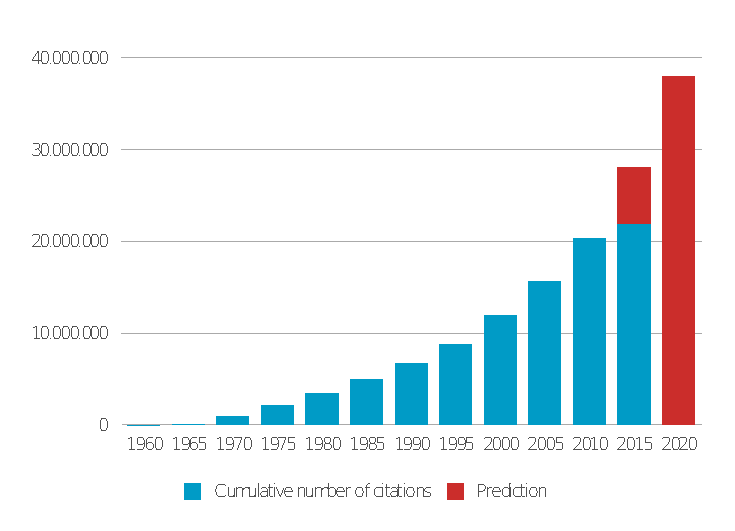
\includegraphics[width=0.8\textwidth]{Figures/Fig1.eps}
  \caption[Cumulative number of MEDLINE citations]{Cumulative number of citations in MEDLINE as shown in \cite[figure 1.1]{wachinger2013next}}
  \label{fig:citations}
\end{figure}

However, currently available text mining systems have only limited understanding of biomedical texts, leading to high error rates when compared to manual analysis (see \cite{rebholz2005facts}). For specific use cases, specialized algorithms\footnote{for example, ChemSpot \cite{rocktaschel2012chemspot} for chemical entity recognition} have been developed in order to provide better recognition characteristics -- notwithstanding the fact that such algorithms are hard to integrate in existing text mining systems that only provide a ready-to-use solution for very narrow use cases.

Moreover, current text mining software is commonly built for analyzing huge text corpora such as the complete set of PMC\footnote{PubMed Central, see \cite{beck2010report}} open access articles. Furthermore, due to legal restrictions, text mining software can only rarely index a large corpus of non-open-access papers -- particularly if the text mining interface is publicly available\footnote{Journal subscription agreements frequently do not include the right of indexing or making the derivative works available to the general public, see \eg the example agreement available at \cite{sciencedirect2012}.}.

No ready-to-use tailored solution is currently available for domain-specific applications: If one intends to analyze only a comparatively small corpus of data -- for instance, scientific publications only about a single bacterium plus a collection of other data sources like laboratory reports in heterogeneous formats -- the user either has to resort to unspecific, non-specialized systems facilitating simple full-text search in arbitrary documents or adapt a complex text mining system with custom algorithms.

When using existing systems like \textit{Excerbt} (see \cite{barnickel2009large} and \cite{wachinger2013next}), not only does the complex high-throughput-oriented architecture lead to difficulties in writing code for importing the documents in question, the system also has significant inherent overheads that require it to run on a high-performance server cluster\footnote{Excerbt 2.0 used 20 servers with a total of 240 GiB of RAM and 160 TiB of harddrive disk space, see \cite[section 4.2.1]{wachinger2013next}.} . Even imports of single documents take up to several hours due to this overhead\footnote{The timeframe of performing a data update in the original Excerbt version has been outlined in \cite[section 4.1]{wachinger2013next}. However, from my previous experience as an Excerbt developer, I know that even computing jobs that did not perform any operation at all took about 30 minutes in the production configuration as present in early 2013.}.

Together with the immense administration overhead inherently present in complex multi-tiered architectures\footnote{During development of Excerbt, the cluster software frequently required full restarts and other maintenance due to unexpected job failures. At the date of writing this thesis, the public Excerbt service \cite{excerbt} is unavailable due to maintenance issues.} this leads to the hypothesis that it would require months to years to setup a customized instance of Excerbt -- even for a single application.
  
Although text mining is an important tool for modern computational biology\footnote{A good overview about practical uses in life sciences in listed in \cite{galvez2008knowledge}.}, its practical applicability is confined by complex software, its inherent focus on large-scale applications and hardware requirements that can't be fulfilled in a small application-specific setup or for a application that requires using the system autonomously without internet connection.

Moreover, as the number of specialized algorithms for text mining application grows continuously, next-generation text mining systems should allow highly customizable modules -- for example, users in the area of chemoinformatics should be able to use application-specific ontologies\footnote{A database or resource of biological entities, see \cite[section 2.5.2]{wachinger2013next}.} with a focus on chemical compounds and structural properties, while another user performing research in algorithmics might need specialized preprocessing that can properly interpret mathematical terminology or even formulas.

What would be required in order to work around these issues is a set of algorithms and tools that can be used in a standalone manner for text mining in \itquote{resource-constrained} environments. This means that commodity  hardware like notebooks -- or even mobile devices like tablets and smartphones -- can be used in place of dedicated server clusters, allowing not only existing hardware being used for this purpose but also facilitating the use of text mining technology where before this was not possible due to the high cost and maintenance effort required to run a cluster.
\newpage
For this thesis, based on my previous experience in engineering the Excerbt system I developed the following seven algorithms to improve search indexing, named entity recognition and client communication for resource-constrained applications:
\begin{itemize}
  \item \textbf{PRIMORDIAL} - \textit{Performant Record Indexing using Merge Operators with Runtime-Delayed Interpretation of Accumulated List operations}, an algorithm for lazy indexing leveraging merge operators, a special feature of key-value databases, for efficient inverted index generation (see section \ref{sec:primordial})

  \item \textbf{PRAISER} - \textit{Partial Reindexing Algorithm with In-place Stable Elimination of Redundancy}, a merge operator for use within the PRIMORDIAL algorithm that exhibits properties allowing stable incremental and partial index generation and featuring automatic removal of duplicate results (see section \ref{sec:praiser})

  \item \textbf{PERSIST} - \textit{Performant Extraction of Results by Set Intersection of Single-Token-indices}, a concept that allows to save the majority of space occupied by inverted search indices by avoiding to create separate index entries for multi-token entries (see section \ref{sec:persist})
  
  \item \textbf{PRESIDE} - \textit{Prefix-based REaltime Search by Iteration of Database Entries}, a schema that allows performant real-time searching for token prefixes in key-value databases that support sequential iteration (see section \ref{sec:preside})

  \item \textbf{PRO-PANE} - \textit{Prefix-based Result Ordering with Programmable Antecedence of End Results}, a key-value database layout augmentation that allows query-level-selectable dynamic result reordering, thereby facilitaing displaying of more relevant search results before less important ones (see section \ref{sec:pro-pane})

  \item \textbf{FiT-NESS} - \textit{FIrst-Token-based Named Entity Selection Scheme}, an optimization of the NER algorithm used by Excerbt that achieves $\mathcal{O}(1)$ index space consumption in respect to the number of tokens in the indexed entities (see section \ref{sec:fitness})

  \item \textbf{WESTSIDE} - \textit{WEbSocket-based STateful Sequentialization of Incoming Data Envelopes}, an algorithm facilitating fast bidirectional browser-to-server communication  that allows using a simple sequential programming model in the server while still maintaining performance benefits of an asynchronous system (see section \ref{sec:westside})
\end{itemize}

These algorithms have been implemented in a proof-of-concept tool called Translatron (TRANSLAtional bioinformatics\footnote{see \cite{butte2008translational}} Tool with Realtime ONtology). Its web-focused architecture allows out-of-the box indexing and real-time search in both documents and ontologies while facilitating high extensibility and integration of third-party algorithms by using a lightweight Python-based implementation.

\chapter{Results}\label{chapter:translatron} 
\setlength{\epigraphwidth}{10cm}
%\epigraphfontsize{\small\itshape}
\epigraph{\textit{If you can land on the moon using a pocket calculator, why can't you do text mining using only your smartphone?}}

As outlined in chapter \ref{chapter:introduction} Translatron has been designed for processing of small to medium text corpora. The new version of Excerbt\footnote{Described in \cite{wachinger2013next}, as opposed to the ``old Excerbt'' initially published in \cite{barnickel2009large}.}, on the other hand, has been designed for processing the entirety of available text sources\footnote{While according to \cite{wachinger2013next} only MEDLINE and PMC are currently imported in the current production version of Excerbt, the system is not inherently limited to those corpora.}, not only including open access sources but also abstracts from non-open-access papers listed in PubMed whose abstracts are available via the MEDLINE service (see \cite{hunter2006biomedical}).

Besides the targeted use cases being different from Excerbt, the user interface (UI) uses an approach called \textit{real-time search}. The search results are displayed directly while typing the search term without the need to press enter, enabling the user to successively refine the search terms based on the observed results. Furthermore, the support for named entity recognition not only allows users to find arbitrary entities in search results but also facilitates a direct crosslinking to additional information about said entity (see section \ref{ssec:ner}).

Python has been selected as a programming language for Translatron because of its popularity and ease of use (see \cite{van2007python}, \cite{king2011top} and \cite{sanner1999python}). As a scripting language, it allows easy modification without the requirement of explicitly rebuilding the software, yet facilitating clean, high-level code that can easily be understood even with little previous experience.

Though it can be argued that Python is slow and might be more memory-intensive when compared to compiled languages like \CC, Translatron is not optimized for pure execution speed but for inherent simplicity and the operation on resource-constrained devices. Should an improved performance be required, one solution would be to use alternative, Just-in-time-Compiler\footnote{a compiler that is capable of runtime interpretation, but uses pre-compilation and runtime optimization in order to gain a performance benefit over pure runtime interpreters.} (JIT) based Python implementations like PyPy (see \cite{bolz2009tracing}). In most other cases, YakDB (the database used by Translatron as discussed in section \ref{sec:databases}) provides sufficient performance benefits due to its highly efficient \CC\ implementation.

\section{Translatron's architecture}\label{sec:translatron-architecture}

\begin{figure}[!htb]
  \centering
  \includegraphics[width=0.8\textwidth]{Graphics/Workflow.eps}
  \caption[Translatron's data import workflow]{Translatron's basic data import workflow}
  \label{fig:import-workflow}
\end{figure}

Similar to Excerbt, Translatron is built on the idea of a basic \textit{import -- indexing -- search} workflow. Besides importing documents, entity import (also called ontology import, see \cite{wachinger2013next}) is also supported, though not required if a specific application does not depend on using the named entity recognition discussed in section \ref{ssec:ner}. A general overview of the data import workflow is depicted in figure \ref{fig:import-workflow}.

Although details of this architecture will be discussed later in this thesis, just like Excerbt Translatron is not a fully standalone program but consists of a stack of tool and libraries. An overview of the design is given in figure \ref{fig:translatron-architecture}. In this diagram, it is obvious that the ``NER / Ontology / Entity'' indexing block is topographically equivalent to the ``Text corpus / Full text search / Document indexing'' block. This is not due to the simplified nature of the diagram but instead reflects the design's reality, because both blocks use exactly the same entity storage and indexing backend, thereby reducing the complexity of Translatron's codebase.

\begin{figure}[!htb]
  \centering
  \includegraphics[width=0.7\textwidth]{Graphics/Translatron-Architecture.eps}
  \caption[Translatron architectural overview]{Translatron architectural overview diagram (simplified)}
  \label{fig:translatron-architecture}
\end{figure}

On the client-side, Translatron uses a purely static web interface (\ie no part of the interface is dynamically generated by the server), making it easier to adapt to custom needs. An AngularJS (see \cite{angularjs} and \cite{darwin2013angularjs})-based frontend easily allows augmenting the interface with additional features without explicitly having to deal with the details of the client-server communication and user interface rendering. The web interface is served via an embedded HTTP webserver -- the client-server communication, on the other hand, is performed via WebSockets as described in section \ref{sec:westside}.

\begin{figure}[!htb]
  \centering
  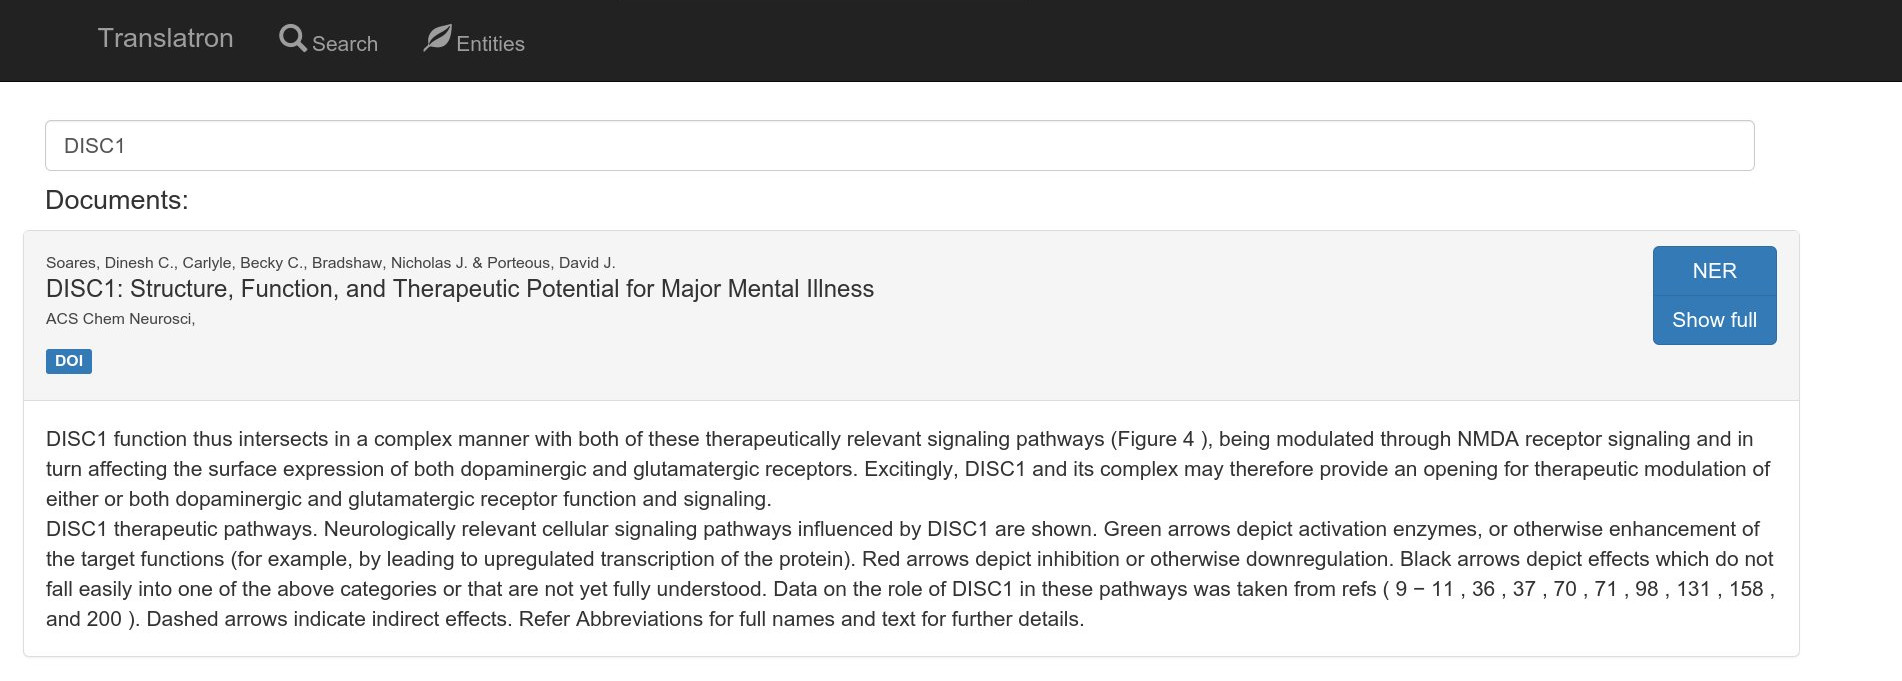
\includegraphics[width=1.0\textwidth]{Figures/Translatron-Search.eps}
  \caption[Translatron search example]{Searching for \itquote{DISC1} in Translatron (screenshot)}
  \label{fig:translatron-search}
\end{figure}

An example search with Translatron is shown in figure \ref{fig:translatron-search} (all search results besides the first one are hidden). While the \itquote{NER} button alongside each search result triggers the named entity recognition feature as discussed in section \ref{ssec:ner}, the \itquote{Show full} button shows the full stored text of the document while by default only the paragraphs around the search hit are shown.

Translatron also allows direct searching for entities as shown in figure \vref{fig:translatron-entities} and discussed in detail in section \ref{sssec:ner-excerbt-translatron}.

\section{Autonomous text mining software - an introductory use case}\label{sec:autonomous-textmining}

While text mining without access to fast internet and virtually unlimited hardware resources seems to be an unrealistic use case for most users that only intend to operate the system from their office, it is entirely realistic to see an application of text mining in disaster relief, \eg after earthquakes. While autonomous text mining systems certainly will only solve a very small subset of the issues encountered by disaster relief personnel, they can be a potentially life-saving tool especially in the context of epidemiology-oriented microbiology. For example, Feldstein and Weiss note in \cite{feldstein1982cambodian} regarding patients treated in a Cambodian refugee camp:
 
\begin{quote}
  \itquote{The availability of bacterial cultures could have eliminated the use of multiple and/or broad-spectrum antibiotics in treating most infections} \cite[discussion]{feldstein1982cambodian}
\end{quote}

While one could argue that bacterial cultures would have helped the authors more than a text mining tool, the publication refers to events dating back to 1980 when no text mining technology even remotely comparable to today's software was available. In fact, text mining may provide additional information that is especially useful when the patient's condition is unclear or ambiguous -- the same reason that led Feldstein et al. to the assertion that bacterial cultures would help in diagnostics and facilitate a better treatment.

Consider the following example: A patient is admitted to a remote disaster relief hospital in a third-world country after a large earthquake. As the communication systems collapsed, only limited satellite-based internet is available for the medical personnel. Said patient's symptoms show clear signs of bacterial infection due to an open fracture suffered from the earthquake. However, based on the symptoms, the doctor -- who has not received specialized training in infectiology -- doesn't know exactly what bacterium might be causing the infection. As the open fracture requires urgent surgery, antibiotics need to be administered immediately. There are many other patients waiting, therefore the doctor has only limited time available for research.

Using Translatron -- which is running autonomously on a smartphone -- the doctor searches for the patient's symptoms in a microbiology/infectiology-specific text corpus based on MEDLINE and PMC. Translatron finds \cite{inglesby2002anthrax}, associating the patient's symptoms to Antrax which is caused by \textit{Bacillus anthracis}. Based on this information, the doctor is not only able to administer suitable narrow spectrum antibiotics but also evaluate possible epidemiological consequences of the case: Fellow doctors are informed of typical symptoms and suitable methods of decontamination -- official authorities can also be involved immediately and take precautionary measures to avoid endemic behavior.

This scenario would not be possible with a system like Excerbt, as fast internet is frequently not available in disaster relief scenarios and a local cluster setup is logistically difficult and time-consuming -- especially if no dry, clean building with sufficient continuous power is available to house multiple servers.

\section{Requirements for resource-constrained text mining}

Due to the different targeted application sets, there are vastly different technological requirements to Translatron as there are to Excerbt. In the following sections the requirements and implementations of Translatron and Excerbt will be compared, focusing on the aspects that seem most relevant for Translatron's use case.

Excerbt has been selected as a base for comparison not only because the development of YakDB and Translatron initially started as a complete redesign of the Excerbt topology and only later focused on specialized text mining applications -- but also, because as being a core developer of the new Excerbt system for more than two years I have access to significantly more details regarding the system design than for other, comparable text mining systems. While many publication tend to hide negative over positive results (see \cite{fanelli2012negative}), I believe that for a complete redesign information about concepts that did not work out as expected are equally important as knowledge about the approaches that succeeded -- to me however, this information is only available about Excerbt, making it an ideal candidate for comparison.

\subsection{Domain-specific text mining}\label{ssec:domain-specific-textmining}

As already discussed briefly in chapter \ref{chapter:introduction}, Translatron -- in contrast to Excerbt and many of its competitors -- is not designed for large-scale \itquote{big data} text mining. This means that while Excerbt has been designed as a large, scalable system that not only supports processing the whole PMC corpus plus MEDLINE but can also easily scaled to support even larger corpora like the entirety of newspapers or English literature.

While the generic approach of scalability at first seems appropriate, it introduces a significant overhead not only in software complexity but also in hardware, rendering the Excerbt architecture virtually useless for heavily resource-constrained devices like smartphones (also see section \ref{ssec:clustering}).

Also, the value of searching huge text corpora is highly disputable: While Excerbt is designed for a single installation to cover all possible use cases, most users only intend to search in a \itquote{domain-specific} subset\footnote{\ie a subset covers a distinct set of topics, the ``domain''.} of the available text corpora. For example, a microbiologist researching virulence of \textit{Coxiella burnetii} is commonly only interested in a subset of the publications related to microbiolog. Giving that user access to specifics about neurological damage due to Alzheimer's disease in mice will rarely be useful.

Moreover, the corpus will likely not be static: While new papers or even internal reports might be added continuously, the user might also remove papers that seem unreliable or are not any more considered relevant for the specific use case. Furthermore, it is possible that some use cases will require either a parallel deployment\footnote{Inherently supported by Translatron, even on the same computer.} or a quick switching\footnote{Supported in Translatron using the backup/restore mechanism as discussed in section \ref{sssec:redundancy-translatron}.} of multiple corpora and ontologies: Besides using a \textit{Coxiella burnetii}-specific deployment, said biologist might have specific queries that require a microbiology-specific corpus (including, but not being limited to \textit{Coxiella burnetii}) that can be used, for example, to find similarities between \textit{Coxiella} strains and other bacteria or to include host-specific information to investigate the host-pathogen interaction

By providing a customizable domain-specific system that can run locally without the need for complex setup procedures, a multitude of use cases without specific restriction can be covered by Translatron. Although there are no hard boundaries on how large Translatron-indexed corpora can get, there are circumstances where extremely large text corpora in Translatron are likely to consume more main memory than available on the device, thus either crashing the software or rendering it slow (also see \ref{ssec:resource-constraints}). Similar limitations apply to Excerbt which handles this issue by simply making use of hardware clusters with an extended amount of main memory.

\subsection{Types of resource constraints}\label{ssec:resource-constraints}

In chapter \ref{chapter:introduction} we introduced the concept of making next-generation text mining software run autonomously\footnote{In the context of this thesis, an autonomous text mining system is defined as a software than can run both offline and online and on an single computing device (including the device displaying the interface to the end-user) without any specific constraint on usage scenarios, provided that the data to be analyzed is available to the system.} on single devices, even down to mobile handhelds like smartphones and tablets. In order to be able to evaluate and compare the capability of Excerbt and Translatron on those devices, it is required to define and discuss the most important classes of resource constraints present on off-the-shelf commodity devices:

\begin{itemize}
  \item \textbf{Main-memory constrained systems}: These devices have a low amount of main memory, also called RAM (random access memory). While servers like those used by Excerbt commonly have main memory between 16 and 192 GiB (see \cite[figure 4.3]{wachinger2013next}), commodity hardware often has less than 8 GiB of RAM. Moreover, even modern handhelds, embedded devices and cheap virtual servers have less than 2 GiB of RAM and even devices with as little as 256 MiB should generally be able to run Translatron, albeit the performance is expected to be worse when compared to more powerful computers.
  
  One platform that has received a significant amount of attention in a wide variety of scientific fields is the Raspberry Pi low-cost embedded Linux system. The Raspberry Pi is a low-cost (around 25\$) single-board computer that only requires a SD card and an USB power supply to run. Due to its compact form factor and its low price, multiple Raspberry Pi computers can be used to form a small, low-cost computing cluster (see \eg\hspace{-.2em}\cite{cox2014iridis}). However, the individual computing nodes of those clusters have at maximum one gigabyte of main memory\footnote{for the new model ``Raspberry Pi 2'', the old version only having 512 megabytes.}, rendering the platform nearly unusable for text mining software that consumes multiple gigabytes of memory even while idle. Although Translatron's performance is considered to be generally better on more powerful computers like notebooks, the Raspberry Pi allows cost-efficient local deployment of a web-based text mining system like Translatron -- the performance penalty inherent to that configuration is considered acceptable for many applications.
  
  \item \textbf{Storage space constrained systems}: Even in server-based systems like the old Excerbt, there are issues with disk space running out due to ever-growing amounts of data (see \cite[section 4.2.1]{wachinger2013next}). While the new Excerbt software stack has been specifically designed to have more than 100 TiB of storage available to the application and to be easily scalable (see section \ref{sssec:clustering-excerbt}), handheld devices only encompass storage space of a few tens of gigabytes, with only a few gigabytes being available to the application. Although smaller domain-specific corpora (when compared to a full PMC/MEDLINE corpus as in Excerbt) automatically lead to significantly decreased space consumption, without specialized algorithms, the available disk space might still be insufficient.
  
  \item \textbf{CPU-time constrained systems}: As a constraint, this constellation is rather rare as there is no inherently limited amount of CPU time as it is the case for main memory or storage space. In cloud computing, there are scenarios where the amount of CPU time consumed indirectly leads to higher costs (see for example the Amazon AWS EC2 price table \cite{ec2-pricing}). Due to the tradeoff of simplicity versus optimization and the requirement that Translatron should be easily extensible, it is not optimized for pure execution speed -- notwithstanding the fact that many aspects of Translatron like the real-time search would not be possible without optimization at some level.
  
  \item \textbf{Network-constrained systems}: The systems affected by this class of constraint are mainly mobile handheld devices or embedded boards like the Raspberry Pi. Those systems have either a slower maximum network connectivity than a reference system and/or exhibit higher latencies. For example, a smartphone that is connected to a wireless 802.11n network has a theoretical maximum speed of 300 MBit/s (with 2 MIMO antennas on both endpoints, see \cite{ieee80211n}). Although the evaluation of wireless network performance is beyond the scope of this thesis, in practice lower speeds and worse latencies are not only achieved due to physical distance between smartphone and access point but also due to the fact that the wireless spectrum is often shared between multiple devices and networks.
  
  Although no authoritative tests have been performed, it is expected that internal network performance is a critical factor for clustered systems like Excerbt. Even more important to the end user is the network connection from the device displaying the user interface to the server instance: A high latency in this path will degrade the performance perceived by the user as the communication poses the bottleneck for viewing search results. While this is generally not a critical issue for local network connections, users in rural areas in foreign countries accessing servers available on the internet will not only experience a slow connection but will also have to deal with connection errors. A comparable use case is discussed in section \ref{sec:autonomous-textmining}.
  
  Translatron has not been particularly optimized for minimum network utilization -- not because network-constrained systems are considered an irrelevant use case, but because the core system design of Translatron completely works around this class of constraints by allowing true offline usage, thereby eliminating network access altogether during normal operation\footnote{Depending on data availability, the input data might need to be downloaded from the internet.}.
  
  \item \textbf{Battery-constrained systems}: This class applies to handheld devices and notebooks in particular: If there is no permanent power supply available and a text mining system continuously drains the battery, the system can only be used for a limited period of time. This is closely tied to CPU usage, network usage and mass storage device usage, as those are the main factors for power consumption -- especially if the network is only available using wide area wireless networks such as UMTS.
  
  It seems likely that in practice the only use case where strict battery constraints are present are handheld devices that are not continuously connected to a power supply for portability reasons. Even for use cases as discussed in section \ref{sec:autonomous-textmining} the medical equipment is likely to require a steady power source like a generator, possibly also capable of providing a small amount of power to the computer equipment.
  
  Therefore, Translatron is not specifically optimized for battery constraints. However, the inherent possibility of true autonomous operation leads to zero required network traffic, in effect reducing the power consumption by Translatron. Even if the Translatron server is not running on the local device, the lightweight system design will lead to reduced resource utilization, effectively reducing the amount of power being used.
\end{itemize}
  
In the context of this thesis, systems that are storage space constrained and/or main-memory constrained are called \textit{space-constrained} where no specific differentiation is required.

In practice, quite often a tradeoff exists between two or more of these constraints: For example, on a notebook, when optimized for battery-powered field use, there is a tradeoff between battery life and networking speed. If Ethernet is used as a networking interface, a \num{1000} MBit/s network configuration consumes more power than 100 MBit/s mode. For example, when using the DP83865-EP physical layer transceiver\footnote{An integrated circuit that is used to convert the digital data from the network controller to an electrical form suitable for transmission via twisted-pair copper cable  or fibreoptics and vice versa.}, it consumes 1.3W\footnote{$0.43A * 1.8V + 0.19A * 2.5V + 0.01A * 2.5V + 0.01A * 3.3V = 1.307W$ active current} while the exact same integrated circuit (IC) in 100 MBit/s mode only consumes 0.33W\footnote{$0.07A * 1.8V + 0.06A * 2.5V + 0.01A * 2.5V + 0.01A * 3.3V = 0.334W$ active current} (see \cite[section 6.10]{dp83865}) -- in other words, just by switching the same hardware to 100MBit/s connectivity instead of \num{1000} MBit/s Ethernet saves almost 75\% of the power consumed by the device, albeit with $\frac{1}{10}$ the maximum throughput rate.

Similar tradeoffs might apply for other pairs of constraints -- a common case is to precompute full search indices in order to speedup searching and thereby trade mass storage space for speed.

\subsection{YakDB - a database for inverted index applications}\label{sec:databases}

One of the most important factors influencing the performance and ease of use of any text mining systems is the underlying database software. Barnickel's original Excerbt used the PostgreSQL database , which -- being a relational database -- allows the direct processing of complex data types in the database itself. However, this approach led to significant performance issues over several years of runtime (see \cite[section 4.5]{wachinger2013next}).

Due to the issues with relational databases, several sets of conceptual alternatives -- commonly called NoSQL -- were evaluated during the early stages of the Excerbt redesign. Different classes of alternatives are discussed in detail in \cite[section 2.4]{wachinger2013next} for the Excerbt use case, detailing the decision process for its system design. Among a multitude of alternatives, a combined solution based on Hadoop, HBase and ElasticSearch was selected, although there were several earlier experimental tests with a slightly different database configuration.

After the Excerbt dissertation was finished in 2013, based on both positive and negative experiences with the setup as used by Excerbt, I started the system design phase for a third-generation text mining system that did not exhibit the weaknesses being observable in Excerbt (some important issue are discussed in section \ref{sssec:clustering-excerbt} and section \ref{ssec:redundancy}). This system -- which became Translatron almost two years later -- required a database as an alternative to the Hadoop / HBase stack which turned out to be resource-intensive and difficult to maintain.

By extensive testing, it soon became clear that in order to provide a simple and extensible yet performant system, a key-value-database -- one of the simplest models of a database that underlies many more complex models -- needed to be used, as all databases with more complex basic models such as document databases could not achieve the desired performance for all use cases.

However, at this time, only large-scale \itquote{big-data}\ key-value databases like Hadoop/HBase were available in a ready-to-use package that fulfilled all the requirements and were available under a suitable license.

Therefore, in early 2014 I started to develop YakDB (Yet Another Key-value DataBase) -- a specialized database built for the increasing demands of modern computational biology and focused on extremely high read and write speeds  even for commodity hardware, sacrificing neither simplicity nor performance with the main tradeoff of having a simple key-value database not capable of processing complex objects by itself.

\begin{figure}[!htb]
  \centering
  \includegraphics[width=1.5\textwidth,angle=90]{Figures/YakDB-Architecture.eps}
  \caption[YakDB table IO routing schematic]{YakDB table IO routing schematic (simplified)}
  \label{fig:yakdb-architecture}
\end{figure}

As being observed by comparing YakDB's architecture in figure \ref{fig:yakdb-architecture} to Translatron's architecture in figure \vref{fig:translatron-architecture}, YakDB's internal architecture is significantly more complex than Translatron's design. This is not actually caused by differences in the granularity of the schematics but by design: By moving most of the complexity of Translatron into YakDB, one can improve the simplicity of the high-level Translatron codebase while still leveraging the performance gained by using the efficient YakDB \CC\ code. For almost any use case of Translatron, it is sufficient to treat YakDB as a black-box database exhibiting several distinct and unique properties, at most changing some configuration parameters.

In order to store more complex data types inside YakDB, there are specifications on how to encode graphs, inverted indices and arbitrary objects in the key-value database model. YakDB provides implementations for those methods in its Python library which is closely integrated into Translatron. For storing objects like documents or entities inside YakDB, Translatron uses the \textit{msgpack} encoder (see \cite{furuhashi2013messagepack}) which provides space-efficient cross-language serialization for arbitrary objects, thereby facilitating the storage of document-specific properties in entities and documents. Although some common properties like \itquote{id} and \itquote{name} are generally used by parts of the software, additional properties can be added, for example to display protein sequences directly in Translatron. The serialized value can thereafter be stored in the key-value database. Because YakDB currently does not provide an optimized solution for indexing specific values in those objects, it is not being considered a true object database.

\afterpage{\clearpage}

\subsubsection{Built on RocksDB}
RocksDB (see \cite{rocksdb}) is a high-speed key-value storage library that is being developed and actively used by Facebook. It was developed as a major upgrade of the LevelDB (see \cite{LevelDB}) project which originated out of Google.
 
By itself, RocksDB is simply a \CC\ library providing one key-value\footnote{In recent versions, the RocksDB project added support for what \cite{wachinger2013next} calls a \itquote{Column-oriented database.}. This feature has not yet been implemented in YakDB.} table which can be only be accessed by a single process at a time. This is obviously useless for most applications. Therefore, RocksDB is rarely used as a standalone solution in computational biology.
 
YakDB wraps multiple dynamically created instances of RocksDB and provides a rich network interface on top of them. This approach not only allows fast random access read/write operations, but also provides automatic sorting by key, facilitating fast sequential scans -- a feature that can be used in algorithms like PRESIDE (see \ref{sec:preside}).

\paragraph{Log-structured merge storage} RocksDB internally uses a log-structured merge (LSM) trees in order to store the database on the disk (see \cite{o1996log}). Thoroughly analyzing database storage structures exceeds the scope of this thesis -- however, a brief introduction is required in order to be able to analyze performance impacts of LSM-based databases:

For magnetic storage media, not only the raw maximum throughput rate of the device is limiting the performance, one also needs to take seek times into account. Usage patterns exhibiting frequent non-sequential accesses cause the hard drive to mechanically move to the new position. As this process is quite slow (see \cite{ousterhout1989beating}), performance is severely impacted by this behavior. This especially impacts random writes as in theory every single write will cause a seek operation on the hard disk\footnote{In practice, while write buffering reduces the actual number of seeks for some usage patterns, high-volume writes still have high seek-induced overhead.}.

Using LSM trees, the data is not directly written into the database, but instead it is collected in a log -- a purely sequential data structure. Once the log has reached a pre-configured size, the data is moved to the main tree structure, providing fast read access times\footnote{In this context, no explicit differentiation is made between different trees like B+ trees or Red/Black trees as a detailed discussion would exceed the scope of this thesis.}. While this approach obviously writes all the data at least once more than the classical approach of writing directly to the tree structure, the write access is mainly sequential, providing a large net performance gain.

Although flash-based media are built so that no mechanical operation needs to take place even for random access writes, due to the structure of modern flash-based media, sequential writes are still faster than random ones (see for example the Samsung 830 series datasheet \cite{samsung830ds} which lists a sequential maximum write speed of 320 MB/s for the 128 GB model, while random access 4kb writes reach a maximum at 120 MB/s\footnote{30,000 IOPS * 4 kb}).

According to a study by Dell, when using mainly sequential workloads, the performance advantage of SSDs does not justify their extra cost (see \cite{dellssdhdd}). While prices for SSDs are expected to drop in the future due to increased mass-production it can safely be assumed that for mainly sequential workloads such as LSM databases, HDDs continue to be a suitable alternative to expensive flash-based storage media at least for the next years.

\subsubsection{Numerically identified tables}
Most SQL and NoSQL databases -- for instance, PostgreSQL -- identify distinct tables by name (disregarding hierarchical structures like databases). For example, a table called \itquote{relations} might contain Excerbt's relations. In contrast, YakDB identifies the tables only by an integral number: For instance, the table 5 might contain PMC documents.

While this might sound like an undesired constraint at first, it not only provides some level of robustness against typing errors in table names but a rather large performance gain. Especially in use cases where many millions of database requests are issued by the clients, in the named-table model every single request causes an evaluation of the table name unless a stateful model is used\footnote{This means that \eg for one database connection, one table is pre-selected. While this approach is possible, it adds additional complexity to the system and therefore increases the likelihood of triggering complex failure modes. Additionally, if the connection performs \eg writes to alternating tables, this method creates significant overhead.}. The YakDB numbered-table model works around this issue by only sending one 32-bit unsigned table numbers with each request\footnote{One exception is the \textit{multi-table write request} which is unimplemented at the time of writing this thesis, but will allow deterministic-order atomic insertion into multiple tables. In this request, every single key-value pair to be written contains a table number marker.}, which can be evaluated with virtually no overhead.
 
\subsubsection{\ZMQ-based networking layer}\label{ssssec:zmq}
The YakDB network interface was built to fulfill four essential requirements:
\begin{enumerate}[label={(\arabic*)}]
  \item Cross-language compatibility
  \item Speed, especially low latency also when communicating locally
  \item Simplicity and statelessness\footnote{\ie no explicit state being tied to a connection to increase the robustness of the system.}
  \item Selectable write progress feedback\footnote{\ie support for modes where the server reports that a specific write has been performed successfully, but also for modes where for performance reasons it is only ensured that the network did not fail to deliver the request to the server.}
\end{enumerate}

Based on these criteria, multiple low-level networking libraries were evaluated. Most systems either supported less than five programming languages (violating (1)) or were built with a strong focus and reliability and therefore traded performance for reliability.
 
 One framework -- a very lightweight transparent communication layer called ZeroMQ (\ZMQ) (see \cite{hintjens2013zeromq} \& \cite{zmq-homepage}) stood out:
  \begin{enumerate}[label={(\arabic*)}]
  \item Supports 46 different languages\footnote{as of 2015-05-07, see \cite{zmq-language-bindings}} 
  \item Not only built for latency and throughput comparable to raw socket communication, but also featuring zero-copy-capable lock-free queues that use a transparent API for inter-thread \& inter-process-communication and communication over the network. Additionally, the model features fully asynchronous network writes, facilitating the programming of highly efficient yet simple to use software.
  \item A fully stateless yet fully routable framing model that only requires copying the content into binary \ZMQ\ frames of arbitrary size
  \item Provides not only a request/reply pattern but also push/pull and publish/subscribe topology (see \cite{hintjens2013zeromq}, also discussed in section \ref{ssec:asynchronicity})
 \end{enumerate}

As shown in figure \ref{fig:yakdb-architecture}, YakDB also uses \ZMQ\ for internal communication. By using the inter-thread \itquote{inproc} mechanism, YakDB can use an actor-based threading model, facilitating an almost lock-free database design (see \cite{hintjens2013zeromq}). However, a detailed discussion of these design decisions would exceed the scope of this thesis.
 
\subsubsection{Asynchronicity support}\label{ssec:asynchronicity}

\begin{figure}[!htb]
  \centering
  \includegraphics[width=\textwidth]{Graphics/Asynchronicity.eps}
  \caption[Asynchronous vs. synchronous communication schematic]{Asynchronous vs. synchronous communication (basic principle)}
  \label{fig:asynchronicity}
\end{figure}

As shown in figure \ref{fig:asynchronicity}, YakDB allows both synchronous and asynchronous writes\footnote{Although technically asynchronous reads are possible, their usage is more complex as the further execution of the program commonly relies on the result of the read request. Therefore, in this thesis only asynchronous write requests are discussed.}. Synchronous writes reduce the likelihood of errors for example due to a file system having reached 100\% disk utilization as the client will wait for an error response from the server before sending more datasets. However, asynchronous writes as shown in figure \ref{fig:asynchronicity} provide a clear advantage in performance as the client will continue to compute the next dataset while the database is writing the last value to the disk.

YakDB implements asynchronous writes using the \ZMQ\ push/pull mechanism. While in the classical request/reply model, the client always expects a response message from the server, in the push/pull mode \ZMQ\ only makes sure that the message is properly delivered over the network.

When using asynchronous communication, it needs to be ensured that \textit{flow control} is properly enabled in the software. When the client constantly computes new datasets to write, the computation might be faster than the network or the processing of the data on the server side. Without flow control, excess data that can't be processed in time by subsequent algorithms will be temporarily stored in the main memory -- at one point potentially exceeding the amount of memory available. Therefore, YakDB uses the \ZMQ\ feature of queue watermarking in order to stop the client from generating new data when a predefined amount of data is already present in the queues. This mechanism is transparent to the programmer as in case of overflow the API will simply not return immediately but instead wait until the queue has free space available again.

Although implemented in many database systems, this approach is particularly advantageous for main-memory constrained systems as there are tight limits on how much memory can be consumed by the software at any given time.

\afterpage{\clearpage}

\subsubsection{Lightweight architecture}\label{sssec:lightweight-architecture}

Due to its focus on resource-constrained devices, YakDB is built as a lightweight system, exhibiting the following core properties:

\begin{itemize}
 \item No installation required: The minimal setup consist of a single executable and a configuration file in the same directory
 \item Configuration-free: No explicit configuration required, default configuration enables all features
 \item Fast startup: Less than 0.1 seconds\footnote{Maximum of 25 runs where a stop request was sent to the server immediately after startup.} on a standard Linux computer
 \item Automatic table creation and setup: Once a table is used for the first time, it is automatically opened using the last table configuration or the configurable global default
 \item Tiny codebase of less than 5200 Source Lines of Code (SLOC)\footnote{YakDB standalone server source lines of code, measured using sloccount 2.26.} plus less than 4200 SLOC Python interface code\footnote{Includes inverted index and graph implementations, measured using sloccount 2.26.}
\end{itemize}

Although not all of those properties are relevant for most applications, it is clear that Translatron's approach of building a lightweight and thereby extensible is also reflected in YakDB. These properties are especially useful when extending the system. For a detailed discussion, refer to section \ref{ssec:extensibility}.

\subsubsection{Transparent compression}

Although efficient algorithms like PERSIST (see section \ref{sec:persist}) significantly reduce the amount of storage space required for any particular setup of Translatron, this reduction is insufficient for many use cases.

Most of the storage space in a typical installation of Translatron being used to mine English texts is occupied by chunks of text and not binary data. According to \cite{shannon1951prediction} and \cite{brown1992estimate} the overall entropy\footnote{Information content in the context of computer science.} of English text is low\footnote{As the exact entropy depends on the corpus in use and potentially other parameters, this discussion uses purely comparative terms instead of quantitative values. ``low'' is defined as entropy where less than 80\% of the space occupied by a symbol is used for encoding information.}. This is quite obvious as English has a very limited character set that is uniformly encoded using \eg an 8-bit ASCII encoding\footnote{For simplicity reasons, the discussion of variable-width encoding methods like UTF-8 including support for foreign language characters is avoided here.} -- therefore some of the eight bits are effectively wasted.

There is a multitude of compression algorithms available that can not only utilize the low entropy of the data stored in the database, but also recurring patterns, for instance common prefixes in a section of the database. The compression used by Translatron is transparent, meaning that the compression is not directly observed by the developer as the database is able to compress/decompress data on the fly and without manual interaction, thus reducing the total amount of disk space occupied by the Translatron database without loss of information.

Although the compression has a potentially negative impact on performance especially for random-access-heavy workloads (as in the worst case, any single access might require a full block of compressed data to be decompressed), Translatron features selectable compression algorithms reaching from high-compression low-speed algorithms like bzip2 to real-time algorithms that can only save a small amount of disk space.

At the time of writing this thesis, the following compression algorithms are supported (see \cite{rocksdb-source}):
\begin{itemize}
 \item No compression
 \item bzip2
 \item Deflate
 \item Snappy
 \item LZ4
 \item LZ4HC
\end{itemize}

For heavily space-constrained devices it is also possible to extend RocksDB to support other algorithms: If space is more valuable than computing time, algorithms like LZMA or PAQ (see \cite{mahoneypaq}) could be used that heavily compress the data and therefore save a significant amount of space when compared with faster algorithms. In principle, it is also possible to implement compression on a dedicated hardware platform to facilitate fast data processing even on low-end devices. However, this approach generally requires a significant effort and is commonly not cost-effective when compared to a solution where more powerful hardware like a notebook is used.

For text mining systems, asymmetrical compression algorithms are particularly suitable. These methods use more computing time for compression than for decompression and therefore are especially suited for applications where data is rarely written but frequently read.

%TODO Stats?

\subsection{Clustered architecture}\label{ssec:clustering}

\subsubsection{Clustering in Excerbt}\label{sssec:clustering-excerbt}

\begin{figure}[!htb]
  \centering
  \includegraphics[width=0.50\textwidth]{Graphics/Excerbt-Architecture.eps}
  \caption[Excerbt architecture]{Excerbt architecture (simplified, see \cite[section 4.2]{wachinger2013next})}
  \label{fig:excerbt-architecture}
\end{figure}

%Why has clustering been added in Excerbt?
The old version of Excerbt, as published in \cite{barnickel2009large}, used only a single server with expensive and small\footnote{1176 GiB in total, distributed over eight hard drives.}, yet fast hard drives (\cite[section 4.2.1]{wachinger2013next}).

\begin{quote}
  \itquote{These are very expensive disks (compared to regular commodity disks, such as SATA) and only available in limited storage capacities because of an exponential proportion of storage vs. price.} (\cite[section 4.1]{wachinger2013next})
\end{quote}

In this version of Excerbt, although the full indexed dataset could fit on the storage, only few tens of gigabytes remained free on the hard drives of the server. Due to architectural limitations of the PostgreSQL database (which was in use in this version of Excerbt, see \cite[section 4.5]{wachinger2013next}) this led to the impossibility of performing certain operations on the database, as those operations require a significant amount of temporary storage space on the hard disk. One of those operations was \textit{VACUUM FULL} which garbage-collects free space inside the table storage of the database and therefore increases overall access speed while decreasing space utilization (see \cite{postgresvacuum}). Due to the inability to perform a \textit{VACUUM FULL} run on the Excerbt tables (which would have alleviated most of the performance issues at that time), both write and access speed were getting increasingly slow, leading to access times ranging up to multiple hours for more complex queries (see \cite[section 4]{wachinger2013next}).

In order to totally avoid these possibilities for the future, during the redesign of Excerbt we started to use a clustered approach based on the Hadoop ecosystem. This configuration uses multiple servers working together as a software-controlled unit to provide reliable and performant services.

% How does Excerbt clustering work

As depicted in figure \ref{fig:excerbt-architecture} (a more detailed architectural diagram of Excerbt is shown in \cite[figure 2.9]{wachinger2013next}), Excerbt mainly accesses the database layer HBase. The underlying Hadoop framework (see \cite{taylor2010overview}) provides a distributed file system layer. Not only does this have the advantage of providing scalable storage space that can be expanded by simply adding an extra server and configuring it to connect to the cluster, it also provides built-in redundancy. This feature is discussed in detail in section \ref{ssec:redundancy}.

\afterpage{\clearpage}

% Why is clustering still not relevant for Translatron?

\subsubsection{Clustering in Translatron}\label{sssec:clustering-translatron}

This leads to the question why Translatron should not also use a cluster-based architecture just like Excerbt. There are several reasons why this approach has not been implemented:

\begin{itemize}
 \item \textbf{Performance overhead}: While clustering often results in a net gain in performance due to the inherent ability to distribute work over multiple independent nodes, it depends on \textit{data locality} in order to avoid overhead by sending data over the network. However, in cases where the amount of overall data to be processed is small and/or only few computing nodes are available, the intrinsic overhead of the system outweighs its benefits. As Translatron is built for a typical use case with only a single node, it is obvious that the classic clustering (as present in Excerbt) will result in an overall decreased performance of the system.
 
 \item \textbf{Increased software complexity:} During Development of the new Excerbt implementation, we encountered several issues due to the complexity of the software stack: Not only did the system require manual configuration of the Hadoop distributed file system server, it also required the cluster coordination software \textit{ZooKeeper} (see \cite{hunt2010zookeeper}). Although both the configuration process and the software itself is well-documented, setting up a testing environment on a single notebook took an entire day during the development cycle and required continuous maintenance. While software like ElasticSearch provides UDP-based cluster autodiscovery and is therefore more likely to work fine without configuration, starting multiple independent instances in the same local network\footnote{Depending on the network configuration, the UDP multicast packets usually don't cross any router boundaries.} causes a cluster to form spontaneously and therefore might cause inadvertent effects in practical environments:
 
 \begin{quote}
  \itquote{Multicast is excellent for development, since you don’t need to do anything. [...]. This ease of use is the exact reason you should disable it in production. The last thing you want is for nodes to accidentally join your production network, simply because they received an errant multicast ping.} (\cite{elasticsearch-config-changes})
 \end{quote}
 
 This leads to the conclusion that cluster configuration either requires significant amounts of work or is likely to inadvertently trigger complex failure modes that are difficult to avoid entirely. Said failure modes tend to cause unintuitive behavior and therefore need to be avoided in Translatron as far as possible.
 
 Moreover, the patent \cite{das2006method} seems to encompass the autodiscovery method used in ElasticSearch. In order to avoid legal issues for all possible use cases of Translatron, using this method appears to be impossible without qualified legal advice which is not available at the time of writing this thesis\footnote{}.
 
 \item \textbf{Translatron supports partial clustering}: Although Translatron's architecture has been specifically designed to avoid the issues we encountered during the development of Excerbt, it still maintains the possibility of distributing tasks like indexing to multiple nodes. However, in its current form Translatron lacks some implementation details that would be required to use YakDB's distributed data processing capabilities -- however, the source code of Translatron is built to facilitate easy understanding, therefore features like this are easy to add.
 
 See section \ref{limitations:clustering} for a detailed discussion on how certain clustering features could be implemented.
\end{itemize}

\newpage
\subsection{Redundancy}\label{ssec:redundancy}

The new Hadoop-based Excerbt architecture provides a built-in feature for data redundancy based on the Hadoop file system \cite[section 4.1 \& 4.5]{wachinger2013next}. However, in order to be able to evaluate objectively whether redundancy is required for a specific use case of a text mining system, we first have to formally define which criteria are relevant to this decision:

\begin{samepage}
\begin{boxedDefinition}[Criteria for redundancy in text mining systems]\label{def:redundancy-criteria}
In the context of text mining systems, implementing redundancy is recommended if at least one of the following conditions apply to the actual scenario:
  \begin{enumerate}[label={(\arabic*)}]
   \item Only limited downtimes are acceptable
   \item Recomputing the data that is stored in the system from the original sources consumes more resources than acceptable
   \item Not all original sources are available within a reasonable timeframe
   \item In case of failure of a system-critical component, restoring the system to a fully operational state consumes more than an acceptable amount of time and/or resources
  \end{enumerate}
  {\setlength{\parindent}{0cm} The constraints ``acceptable'' and ``limited'' need to be evaluated in an application-specific way.}
\end{boxedDefinition}
 \end{samepage}

\subsubsection{Redundancy in Excerbt}\label{ssec:redundancy-excerbt}
Excerbt is not officially considered a finished product so criterion (1) (see definition \ref{def:redundancy-criteria}) does not apply\footnote{If (1) would apply, other factors besides hardware failure modes are likely to be limiting to the overall reliability. This hypothesis is supported by the fact that at the time of writing this thesis, the public Excerbt service at \cite{excerbt} is unavailable due to software issues.}.

Therefore, the decisive factors for Excerbt are (2), (3) and (4): Recomputing all data in an Excerbt instance encompassing the entire PMC and MEDLINE corpora plus optional extras requires days to weeks, depending on the current cluster health\footnote{Our experience in developing Excerbt showed that the Hadoop/HBase version in use tends to a) increase arbitrary, apparently acausal error frequency and b) degrade overall performance significantly if specific usage patterns are applied and the cluster is not restarted frequently. Although the exact mechanisms involved remain unclear, there are indicators suggesting at least a part of the failure mode is related to Java memory management issues (also see section \ref{sssec:memory-management}). How much a cluster is currently affected by these effects is defined as the \textit{cluster health}.}.

While (3) does not strictly apply to the Excerbt use case, Excerbt archives all documents and has built-in mechanisms to be able to track different version of the same document. However, these mechanisms are currently unused as there is no actual application for Excerbt requiring exact version tracking. Nonetheless it is possible to integrate data sources into Excerbt that are not available for re-indexing in the database, \eg streaming Twitter messages in real-time directly to the indexer.

Requirement (4) is especially important for most practical use cases, because a limited amount of administration time is available for any deployment of the software. Therefore, care is taken during the system design phase so restoring the system in case of hardware failure is easy or -- in the best case -- fully automatic. As magnetic hard drives tend to be the most frequently failing part of server-based clusters (see \cite{pinheiro2007failure}), most systems are built to survive one or more concurrently failing hard drives and automatically recover when said drives are replaced.

Classically, RAID (Redundant Array of Independent Disks) arrays have been used to provide drive-level redundancy. However, newer designs like Hadoop can utilize JBOD (Just a bunch of disks) \footnote{Any disk array which is not connected in a RAID configuration.} yielding improved performance when compared to RAID (see \cite[chapter 9]{white2009hadoop}) due to optimized allocation algorithms that utilize separate disks by themselves\footnote{\cite{white2009hadoop} therefore recommends to disable RAID for Hadoop servers.}.

Hadoop (and thereby Excerbt) uses a replication-based redundancy mechanism that distributes replicas of data blocks to different servers. This approach theoretically allows fully automatic recovery even in case of multiple concurrent hard drive failure.

\paragraph{Faster processing due to redundant data}

Additionally, this method leads to performance benefits for some usage scenarios: As a single block\footnote{The term \itquote{block} is used in its general meaning here and is not used synonymously to the Hadoop data block as defined in \cite{white2009hadoop}.} is present on multiple nodes, the likelihood that a computing job run can utilize data locality is proportional to the number of replicas (also called the \itquote{replication factor}), provided that each replica is placed on a different node.

This is especially important for computing jobs where the processing time of each block varies significantly from block to block. If initially only local data blocks are processed, some computing nodes are likely to finish processing their local dataset earlier than others. In order to minimize the total job duration, those nodes need to fetch additional datasets from other nodes that have not yet finished processing.
For example, consider an Excerbt instance where an inverted index is being built from PMC documents. Unless the PMC documents are randomly distributed over the data blocks, some blocks will likely contain PMC documents with many figures while others will encompass documents with fewer figures and more text. As figures are not interpreted by Excerbt but consume a significant amount of space, the amount of computational work required for building a full inverted index is significantly higher for the text-heavy PMC documents than for the image-heavy ones.

If, due to replication, the queued data blocks are already present at one of the available (\ie non-occupied) computing nodes, the system's scheduler can use this node to process the block without overhead due to data transfer. This effect matters most when the network is slow compared to the computation. For example, if one megabyte of transferred data requires one hour of computing time to process, a transfer duration of one second would only add $\frac{1}{3600} \approx 0.03\%$ of overhead.

In text mining software, the most time-intensive jobs like SRL (Semantic Role Labelling, see \cite[section 4.4]{wachinger2013next}) tend to exhibit this asymmetry as their processing time depends on a variety of heavily variable parameters like sentence length. Therefore, it can safely be assumed that practical text mining applications will actually exhibit measureable performance benefits if the replication factor is chosen sufficiently high.

\subsubsection{Disk space overhead by replication}\label{sssec:replication-disk-overhead}

Although some asymmetrical workloads profit from a high replication factor, the space consumed by a data block being replicated across multiple nodes is a significant contribution factor for the high disk space consumption of systems like Excerbt. The overall space consumed by a single data block can easily shown to be equal to:

\begin{align}\label{eq:blocksize}
\begin{split}
 S(b) &= |b| * r(b)\ \forall\ b \in B\\\\
 \text{where~} S(b) &: \text{total space occupied by data block $b$}\\
 |b| &: \text{Size of a single copy of data block $b$}\\
 r(b) &: \text{number of replicas $=$ replication factor for block $b$}\\
 B &: \text{The set of all data blocks}
\end{split}
\end{align}

{\setlength{\parindent}{0cm} From equation \eqref{eq:blocksize} it trivially follows that:}
\begin{align}\label{eq:blocksize2}
S(b) &\propto r(b)\ \forall\ b \in B
\end{align}

The key requirement for the proportionality in equation \eqref{eq:blocksize2} is a static replication factor, \ie it does not change over time for any single data block.
Although dynamic, \ie non-constant replication factors are supported by Hadoop, it is not common to have replication factors changing over time. There are use cases, however, where certain sets of blocks have a different replication factor than others. For instance, temporary files containing intermediary results may have a lower replication factor than the main database as they are comparatively easy to recompute.

\subsubsection{Network overhead in replication}\label{sssec:replication-network-overhead}

Although asymmetrical workloads might incur less network traffic due to inherently present data locality (as discussed in section \ref{ssec:redundancy-excerbt}), the process of replication itself has a significant impact on overall network traffic:

Assuming that blocks are only replicated to physically separate, network-connected nodes\footnote{as opposed \eg to replications to separate hard disks on the same node.} and a replication factor of 3, a 100 MiB data block that is present on a single node generates network traffic in excess of 200 MiB. Additionally, if a node or one of its hard disks fail, the blocks stored on the defective disk need to be mirrored to another node, depending on the system hardware causing network traffic of multiple hundred gigabytes.

One important observation is that replication can generally happen asynchronously. Although the system is only fully redundant if every block is has the full number of replicas at any given time, the replication takes a significant amount of time, especially if large amounts of data need to be replicated

It is, however, not necessary to perform these tasks during the computing job that generates the data blocks. The scheduler can perform both replication and cluster balancing\footnote{Ensuring that every node has approximately the same disk utilization, see \cite[section 7]{white2009hadoop}.} when no job is currently active, thereby using the idle time of the cluster that would otherwise be wasted.

\subsubsection{Redundancy in Translatron}\label{sssec:redundancy-translatron}

Translatron has a significantly different set of base requirements than Excerbt, therefore the criteria for redundancy (see definition \vref{def:redundancy-criteria}) need to be evaluated separately:

As Translatron targets different application-specific use cases, criterion (1) might apply depending on the application. However, just like in Excerbt, Translatron itself will likely limit the overall reliability of the system and needs to be tested and modified extensively to meet guaranteed downtime demands.

In contrast to Excerbt, (2) does generally not apply because Translatron is built for small to medium sized datasets. Therefore, the amount of time required to recompute the entire set of data is expected to be several orders of magnitude less than for large-scale big-data-oriented systems like Excerbt.

Regarding criterion (3), however, the situation is similar to Excerbt: While currently no data source is implemented that can't be easily re-downloaded from its original source, due to the good extensibility (as discussed in section \ref{ssec:extensibility}), adding importers for uncommon application-specific data sources is significantly easier when compared to Excerbt. Therefore, it is easy to conclude that there might be applications that depend on the guaranteed data retention in Translatron alone.

Likewise, criterion (4) applies also to Translatron -- however, due to the significantly decreased overall amount of data compared to Excerbt, there is a broader variety of solutions available. Not only does the overall simplicity of Translatron reduce the maintenance overhead but also it is possible to \eg just perform an incremental backup every two hours. With Excerbt, on the other hand, the sheer amount of data stored in the system makes frequent-backup-based approaches virtually impossible to implement.

Based on the observations of section \ref{ssec:redundancy-excerbt}, it is obvious that the replication as implemented in Excerbt is not suitable for the resource-constrained applications targeted by Translatron:

\begin{itemize}
 \item In many use cases targeted by Translatron, only a single device commonly built from commodity hardware is available. This device fulfills the roles of both client and server. Redundancy generally makes no sense on devices with a single mass storage device	.
 
 \item The high disk-space overhead, as discussed in section \ref{sssec:replication-disk-overhead}, is generally not acceptable for space-constrained devices. That means, the replication factor $r(b)$ must be set to $r(b) = 1$, effectively rendering the concept of replication useless while the overhead and the complexity of the implementation is still left behind.
 
 \item In applications where multiple devices are present, network traffic (see section \ref{sssec:replication-network-overhead}) is frequently more expensive than in a scenario with a dedicated cluster like Excerbt. Possible reasons for this include slow network connections (\eg 100 MBit/s Ethernet instead of 10 GB/s fiber-optic Ethernet) or limited battery life (even efficient 1,000 MBit/s Ethernet transceivers consume 1.3 Watts (see section \ref{ssec:resource-constraints}).
 
 \item The implementation of clustering and redundancy is complex. Hadoop 2.7.0 -- the most recent stable version at the time of writing this thesis -- contains about 1.74 million lines of source code\footnote{Measured on a fresh download of the Hadoop 2.7.0 source on 2015-05-05 using sloccount 2.26. Cited number: Total physical lines of source code (exact value: \num{1736088}).}. While Hadoop contains more functionality than just clustering and replication, large codebases are not only likely to contain more critical bugs (see \cite{gaffney1984estimating}), they also limit the extensibility of the system (see also section \ref{ssec:extensibility}). Users extending the system or trying to fix bugs in the code need to understand significantly more code than a user modifying the compact less than 15000 SLOC Translatron + YakDB-codebase (also see section \ref{sec:databases}).
\end{itemize}

This leads to the conclusion that a novel, lightweight, overhead-free and completely optional solution for redundancy needs to be developed. The approach pursued by Translatron is based on YakDB's YDF dump format, whose binary format is specified in appendix \ref{appendix:ydf}. This approach facilitates not only network-capable $\mathcal{O}(1)$-memory highly compressed streaming backup and restoration, but also employs fully atomic snapshotting -- thereby facilitating live (yet entirely consistent) backups even when write-heavy jobs are running concurrently. Other aspects of this behavior are discussed in section \ref{ssec:mapreduce}.

Using this mechanism, it is also possible to implement a workflow where the indexing / import is performed on a server, whereas the mobile handheld devices the Translatron webserver runs on only import dumps from this server. Not only does this circumvent the issue of indexing or import being resource-intensive when compared to just running the server, it also facilitates a centralized management of datasets.

\subsection{MapReduce \& distributed data processing capability}\label{ssec:mapreduce}

\begin{figure}[!htb]
  \centering
  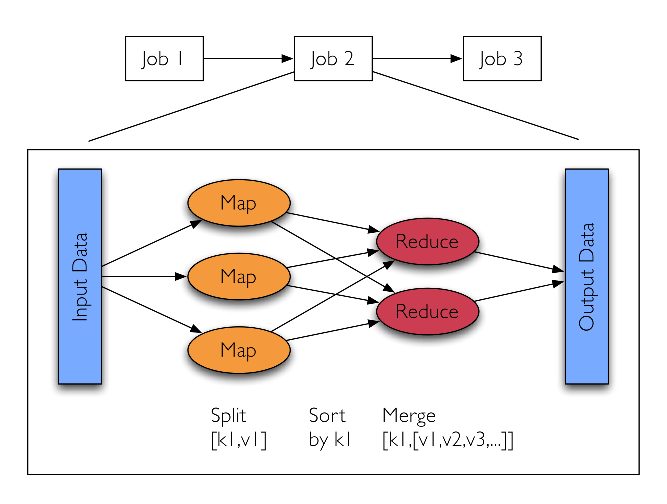
\includegraphics[width=0.60\textwidth]{Figures/Fig25.eps}
  \caption[MapReduce overview]{Overview of the MapReduce paradigm as shown in \cite[figure 2.5]{wachinger2013next}}
  \label{fig:mapreduce-overview}
\end{figure}

MapReduce is a paradigm and algorithm originally developed by Google for their need to process large quantities of data in a distributed manner. By using three phases (\textit{Map}, \textit{Sort} and \textit{Reduce}) to execute an algorithm on a dataset, MapReduce can process up to petabytes of data on large clusters. This is possible because many algorithms can only be efficiently distributed to a large number of computing nodes if they are split into Map/Reduce functions \footnote{A detailed discussion about the reasons for this would exceed the scope of this thesis, refer to \cite{dean2008mapreduce} for details.}. An overview of the paradigm is depicted in figure \ref{fig:mapreduce-overview}  where it is clearly visible that a communication between the nodes only occurs after the map phase and after the reduce phase.

The capability of Translatron to process data using MapReduce algorithm is closely tied to YakDB's capability of processing datasets using MapReduce.
When comparing YakDB to Hadoop, it is immediately obvious that both follow different approaches: While Hadoop is a full-featured distributed processing framework encompassing its own Application Programming Interface (API) for MapReduce, YakDB is a network layer (refer to section \ref{sec:databases}) for the underlying RocksDB key-value database -- therefore by itself possessing only very limited data processing capability.

Although it is planned to extend YakDB with a standalone MapReduce layer and distributed storage capabilities, Translatron -- as of writing this thesis -- only provides the capability of distributing a selectable region of the database to an arbitrary number of clients requesting the data from YakDB while the database guaratees any data block will be sent to exactly one client. However, it is required to manually start worker processes on arbitrary nodes on the network. Those workers can simply write theur output data back to a YakDB table.

This approach allows automatically snapshotting the input dataset using a Copy-On-Write\footnote{The snapshot does not cause a full copy of the database, instead the data at the time of taking the snapshot is kept until the snapshot is destroyed, while newer data that would overwrite the snapshotted data is logged separately and merged on snapshot destruction.} (COW) based mechanism and is also used for generating database backups (refer to section \ref{sssec:redundancy-translatron} for details on the backup mechanism).

By using snapshots for jobs, the system has the inherent advantage that writes to the input table during the job are not reflected in the input job's data -- for example, if a job deletes a region of the input table, said section will still be iterated over by the input table. Though HBase implements a comparable concept called ``versions'', it has been designed to permanently store a number of revision for each value in the database (see \cite[chapter 9]{george2011hbase}). Although there are different use cases where the timestamped versioning as implemented in HBase might be useful, the index model in use by Translatron does not depend on timestamps. Should an application require explicit timestamping, this is easy to implement by appending the timestamp to the key as stored in YakDB. Although this means one needs to cleanup old versions manually when some preset version limit for a single key is reached, avoiding to use optional concepts like versioning decreases the overall complexity of the system.

Although supporting neither a dedicated MapReduce API nor direct spawning\footnote{The process of starting worker processes on nodes in a cluster context} of worker processes on distributed computing nodes increases the effort required to adapt existing MapReduce algorithms, Translatron generally has an easier programming interface by not forcing developers to use MapReduce for tasks where the paradigm provides no benefit. This is the case \eg for very fast, small jobs where the overhead resource consumption associated with the Hadoop model is large when compared to the overall resource consumption of the job itself.

One application where the MapReduce implementation as used by Excerbt would not be applicable is real-time data processing. As even no-operation jobs (\ie jobs that only discard the data without performing any operation on it) that run on an empty section of the database took about 20-30 minutes in the production setup of Excerbt as present in late 2013, it is obvious that one cannot use Hadoop's MapReduce for real-time data processing.

Although one could argue that newer version of Hadoop and HBase could significantly improve this behavior, Hadoop has to make more tradeoffs for other applications due to its complexity and multitude of features. This reduces the likelihood that any particular set of performance issues will be resolved completely, as the solution might impact other applications negatively or destroy compatibility. Additionally, Java-based software has inherent lower boundaries for efficiency: As Hadoop spawns worker processes as completely new Java processes, these first have to interpret large bytecode libraries in order to be able to communicate with the Hadoop ecosystem and run the MapReduce code.

Although there is continuously ongoing research on the optimization of JVM (Java Virtual Machine) based architectures (see for example \cite{inoue2012adaptive}), the garbage-collection\footnote{A set of algorithms that can purge unused variables from memory.} based memory model of Java has frequently exhibited high resource consumption for some MapReduce jobs implemented in Excerbt\footnote{For some workloads, multiple gigabytes of memory per node being consumed and multiple tens of percents of CPU time being utilized have been observed.}.

The memory issues became especially apparent if one job created a large amount of intermediary objects. If a large number of unused small objects in memory are not rapidly discarded, they will not only consume memory for an extended amount of time but also create additional work for the garbage collector.

Obviously, even the possibility of having large memory overhead significantly reduces the applicability of the Hadoop architecture for resource-constrained devices. The YakDB / Translatron stack was designed specifically to alleviate the impact caused by the general problem of memory overhead and does not use the JVM as a basis for its stack.

\subsubsection{Overhead-free programmable data processing}\label{sssec:llvm}
Though not implemented at the time of writing this thesis, there are plans of directly supporting soft real-time data processing in YakDB by utilizing the LLVM framework (Low-Level Virtual Machine, see \cite{lattner2004llvm}), acting as a JIT compiler to run user-defined code. This allows virtually overhead-free processing as data that is read from the database can be passed directly to the user-defined code without first sending it over the network.

Even if the LLVM data processing mechanism is not used, YakDB provides inherently improved communication efficiency by using Unix Domain Sockets as opposed to TCP connections when both the search server\footnote{In general, the part of the software that directly communicates with the database.} and the database run on the same computer. From the benchmark data published by Wright et al. in \cite{wright2007performance} it can clearly been deduced that Unix Domain Sockets not only yield higher throughput and exhibit lower latency but also provide a lower-overhead alternative to local TCP communication.

Although text mining applications only infrequently transmit large amounts of data and therefore it is unclear whether this performance gain is relevant, especially in the import- and indexing phases significant traffic is generated between the database and the indexing software. Battery-constrained devices might therefore profit from an overall lower CPU load and/or faster indexing.

For non-local communication, YakDB is able to use both TCP and Unix Domain Sockets transparently, facilitating fast and overhead-free local communication while concurrently allowing networking. Current version of Java do not support Unix Domain Sockets at all\footnote{Adding support via a 3rd party library would introduce more overhead, possibly eliminating the additional performance gained by using Unix Domain Sockets.} (see \cite{javaforum-unixsockets}).

\subsubsection{Memory management}\label{sssec:memory-management}

Although Java can also be seen as a JIT compiler, it imposes certain restrictions on the user -- for instance, only automated memory collection is supported. LLVM is a complete redesign that allows to use languages with both manual and automated garbage collection. The latter option essentially frees the developer from the responsibility of managing memory in a manual way -- thereby reducing the likelihood of memory leaks. However, depending on the exact garbage collection algorithm in use, some memory usage patterns can yield extremely high overhead as already outlined in section \ref{ssec:mapreduce}. Due to the easier programming approach, however, the development cycle durations using languages with support for automated memory management are frequently less than when using low-level languages with manual memory management.

Although manual memory management generally requires more careful development due to the higher likelihood of memory leaks, a properly written software can leverage the significantly decreased management overhead not only in CPU time consumed by the garbage collector but also in memory that is not freed at the earliest possible point in time.

Based on these observations, it is clear that a flexible system must allow end users to choose virtually arbitrary programming languages not only for writing new software extending the system but also for the integration of existing algorithms. Although Hadoop provides mechanisms like Thrift (see \cite{thrift}) as an inter-language communication protocol, those mechanisms introduce additional layers to the software stack and therefore often incur a significant amount of overhead\footnote{While there seem to be no authoritative benchmarks, the heavily serialization- an deserialization-oriented architecture of tools like Thrift sets a lower boundary on the overhead.}.

\subsection{Extensibility}\label{ssec:extensibility}

As discussed in the previous sections, with Translatron targeting a multitude of possible use cases, it needs to provide the flexibility of being able to not only import custom data in application-specific formats, but also adapt customized algorithms to the software without significant effort.

This requirement also needs to be seen in relation to resource-constrained devices. It can easily be argued that a system like Excerbt employing five\footnote{Hadoop, HBase, ZooKeeper, Excerbt \& ElasticSearch.} distinct and complex software components has not only too many complex failure modes limiting the applicability but also consumes too many resources even to be run on space-constrained devices.

Although Wachinger claims in \cite[section 7]{wachinger2013next} that Excerbt can easily be extended, anyone trying to extend it with additional functionality has to deal not only with the complexity of the architecture (see \cite[section 4.2]{wachinger2013next}) but also with more than 50000 lines of source code\footnote{Measured on a copy of Excerbt's source code from October 2012 using sloccount 2.26, including both the core Excerbt repository and the Excerbt webserver repository.}. While it can be argued that virtually no extension project would require reading the entire source code, it is likely that due to the complexity and the multi-layer stack as in use by Excerbt the time required for familiarization with the system is significant, especially if one has to overcome shortcomings of the system by modifying the core source code.

Translatron achieves higher extensibility than Excerbt using three core properties:
\begin{itemize}
 \item Small codebase: Less than 1500 source lines of code\footnote{Measured using sloccount 2.26, not including YakDB source code.}
 \item Easy-to-understand Python codebase without heavy optimizations that would make the code hard to maintain
 \item Focus on features that are required to fulfill its core purpose, rather than implementing any conceivable set of algorithms
\end{itemize}

Examples where the extensibility facilitated by Translatron can be useful include:
\begin{itemize}
 \item Use of a custom tokenization function\footnote{A function that splits sentences into words or comparable fragments.}
 \item Importing custom text corpora or ontologies or implementing application-specific import filters
 \item Using custom coloring of NER search results (see section \ref{ssec:ner} for a discussion of the NER concept and section \ref{sssec:ner-excerbt-translatron} for a description of coloring in Translatron's NER implementation)
 \item Implementing a modification of the NER algorithm to find special types of fuzzy entity matches such as IUPAC identifiers
 \item Adding support for relation extraction as implemented in Excerbt
 \item Accessing the WebSocket-based interface (see \ref{sec:westside}) programmatically to integrate Translatron's NER into a distinct product
 \item Integrating a user interface that allows switching between different domain-specific corpora or ontologies (see section \ref{sssec:domain-specific-ontologies}) with as little as one click.
 \item Implementing machine-learning based algorithms that automatically import heterogeneous content like web resources or papers in the PDF format
 \item Customizing the stopword list or implementing an algorithm that automatically determines stopwords based on word semantic role and frequency
\end{itemize}

\subsection{Named Entity Recognition}\label{ssec:ner}

One of the core features of both Excerbt and Translatron is Named Entity Recognition (NER), a process where names of real-world concepts or objects are recognized to be present in an arbitrary text. For example, in the sentence \itquote{BRCA1 causes breast cancer}, a NER algorithm could recognize the entity names \itquote{BRCA1} and \itquote{breast cancer}.

After an entity name has been shown to occur at a specific location in said text, one can easily associate it to information available about that entity in existing databases and therefore present augmented information to the user (see \cite{nadeau2007survey}).

There are two general approaches to NER algorithms:

\subsubsection{Pattern-based NER}

If no complete predefined set of entities to search for is available, approaches like machine learning can be used to recognize entities based on patterns specific \eg to a class of genes. Because entities found by pattern-based algorithms can't immediately be associated to a specific entity as present in a database, the hits also need to be classified based on exact match and context (see \cite{nadeau2007survey}).

For applications in life sciences this approach is used by systems like \textit{ChemSpot} (see \cite{rocktaschel2012chemspot}) in order to recognize chemical and biochemical entities including those which are not listed in databases like PubChem (see \cite{wang2009pubchem}).

\subsubsection{Dictionary-oriented NER}

While pattern-based approaches allow recognizing hits not being present in any database, it is difficult to associate previously known information with pattern-based hits because the relation to existing database entries is either unknown or no such database entry exists at all.

Additionally, using fuzzy matching or machine-learning approaches for entity recognition introduces additional uncertainties. While false negative hits can't generally be avoided in NER applications due to factors like spelling discrepancies, semantic ambiguities or literal errors, fuzzy NER algorithms also introduce comparatively high probabilities for false positives (\cite{leaman2008banner} provides exemplary benchmarks of different implementations).

Many applications only require recognition of entities like genes or proteins, for which large databases are available. For instance, UniProt (see \cite{uniprot2008universal}) provides a comprehensive database for proteins including potential cross-references if available.

By indexing protein names and aliases from those databases, one can easily identify matches by just comparing entity names to the  tokens present in the text.

As outlined by Wachinger in \cite[section 4.3]{wachinger2013next}, Excerbt uses dictionary-oriented NER approach using multiple different databases as entity sources (as listed in \cite[table 4.3]{wachinger2013next}). In addition to Translatron's scope, EXCERBT also performs relation extraction and therefore applies the NER to Predicate-Argument-Structures (PAS, see \cite[section 2.5.4]{wachinger2013next}) structures instead of to splitted sentences. Translatron only performs NER on the sentence level (refer to \cite[figure 4.5]{wachinger2013next}) without evaluating SRL information. While this obviously does not allow direct relation extraction, it avoids slow SRL runs while keeping the system design simple to facilitate high extensibility (also see section \ref{ssec:missing-semantic-features}).

\subsubsection{Search modes}
\label{sssec:nersearchmodes}

While many entity types like genes and proteins require\footnote{The requirement depends on the application, but in its standard configuration, Translatron uses Excerbt's model of search types, see \cite[section 4.5, table 4.1]{wachinger2013next}.} exact, case-sensitive search, some entities like MeSH (Medical subject headings, see \cite{lipscomb2000medical}) terms require a case-insensitive search mode.

For example, both variants \itquote{prion diseases} and \itquote{Prion diseases} should be associated to the corresponding MeSH entry when found in the text, whereas \itquote{BRCA1} but not \itquote{brca1} should be associated to the corresponding gene as the latter one is not generally considered a valid notation for the standardized gene identifier.

Additionally, tools like Excerbt also supports other search types like stemmed indexing (see \cite[section 4.3 \& section 4.3.1]{wachinger2013next}). These functions are applied to both the search term and the corpus and therefore allow to alias between natural language variants like \itquote{disease} and \itquote{diseases}, \ie for certain search types. However, as its name suggests, stemming reduces every word to its stem and therefore might not differentiate between notations with semantically different meaning such as \itquote{disease} and \itquote{diseased} (see \cite[section 4.3]{wachinger2013next}).

Furthermore, as described by Porter in \cite[section 3]{porter2001snowball}, stemmers introduce errors due to over-stemming and mis-stemming which can only be solved by using dictionaries to account for special words that need to be stemmed in a certain way.

In order to solve some of the errors introduced by pure stemming methods, Excerbt uses a custom \textit{inflection} algorithm that reduces words to their base form instead of their stem (see \cite[section 4.3, page 79]{wachinger2013next}).

The \textit{BANNER} system (see \cite{leaman2008banner}) also uses an extended stemming algorithm called lemmatization as introduced in \cite{vlachos2007tackling}. \cite[section 3]{leaman2008banner} describes it as
\begin{quote}
\itquote{[...] which is similar in purpose [to stemming] except that words are converted into their base form instead of simply removing the suffix.}
\end{quote}
which is remarkably similar to the description of \textit{inflection} in \cite[section 4.3]{wachinger2013next}:
\begin{quote}
\itquote{An inflector simply reduces every word to its base form instead of the word stem.} 
\end{quote}

In the literature, the term \textit{lemmatization} seems to be used more often in the computation linguistics context (see \eg \cite{liu2012biolemmatizer}, \cite{paulussen1992dilemma} or \cite{Lezius1998}), whereas \textit{inflection} is more often used as a property of certain linguistical forms (\eg \itquote{inflected}) languages (for instance in \itquote{language with rich inflection}, see \cite{abacha2011medical}).

Based on \cite[section 2.2.4]{manning2008introduction} this leads to the conclusion that \textit{inflection} is indeed referring to the opposite process -- variating a word based on its \textit{lemma} or \textit{stem} -- whereas \textit{lemmatization} is the correct term for the base concept of the Excerbt NER search mode.

Although it is likely that subtle differences exist between the Excerbt inflector and previous work in lemmatization algorithms, systems like Excerbt could profit from the integration of improved search modes.

\subsubsection{NER in Excerbt and Translatron}\label{sssec:ner-excerbt-translatron}

Excerbt implements (see \cite[section 4.3.1]{wachinger2013next}) two different forms of named entity recognition:
\begin{itemize}
 \item \textit{Sentence token index (STI) based NER} where entities are searched in an index of documents, see \cite[section 4.3]{wachinger2013next})

 \item \textit{Percolating NER}, where fragments of documents are searched in an index of entities, see \cite[section 4.3.1]{wachinger2013next}
\end{itemize}

It is obvious that when incrementally adding a single document to the database, the STI-based approach requires a full re-run of the named entity recognition software. This is the case because the newly added document might add new search results for the entities\footnote{While one could design an algorithm that only searches the entities in the newly added document, this approach has not been implemented in Excerbt.}, thereby significantly increasing the overhead when the text corpus is not static. Additionally, during the earlier stages of development of the new Excerbt, we faced the challenge that for frequently-mentioned entities like \textit{BRCA1} the search software consumed large amounts of main memory due to the fact that many search engine libraries like Katta (see \cite{katta}) are based on the assumption that a only a small subset of a search results is actually used and will therefore fit into memory. However, in the STI NER, a potentially large list of documents is returned when searching for a common entity in a large corpus. Although this challenge could be solved by using a modification of Katta's backend code, memory consumption by STI NER still presents an issue when being used with large corpora and ontologies.

The percolating NER approach works around this concept entirely by indexing entities instead of documents. Especially for large text corpora, the entity index is significantly smaller than the document index, even if large ontologies are being used. Therefore, in comparison with the STI NER, the percolating approach can also be used on resource-constrained devices.

\paragraph{Translatron's NER}
In Translatron, a variation of the percolating NER is implemented. Using the \textit{FiT-NESS} algorithm as discussed in section \ref{sec:fitness}, further optimization is achieved using an approach allowing entities consisting of multiple tokens to be indexed by only their first token.

This approach facilitates a real-time NER that can be applied to arbitrary texts -- \ie not only those that are imported into Translatron as documents. In conjunction with the real-time search engine, NER is implemented using an \textit{on-demand} approach, where the user has to actively request NER for a document shown as search result. While this might sound unintuitive at first, this means that the system does not have to perform NER for all displayed search results. This is especially important as the NER implementation in Translatron has been optimized for resource-constrained devices rather than for pure execution speed.

Moreover, it is possible to apply the NER algorithm to arbitrary texts. Although not implemented in the user interface, it is possible to use programmatic WebSocket access to send arbitrary text fragments to the server's NER implementation. In fact, the web interface simply takes the currently displayed portion of the search result and sends it to the server using the exact same mechanism.

\paragraph{NER coloring}

\begin{figure}[!htb]
  \centering
  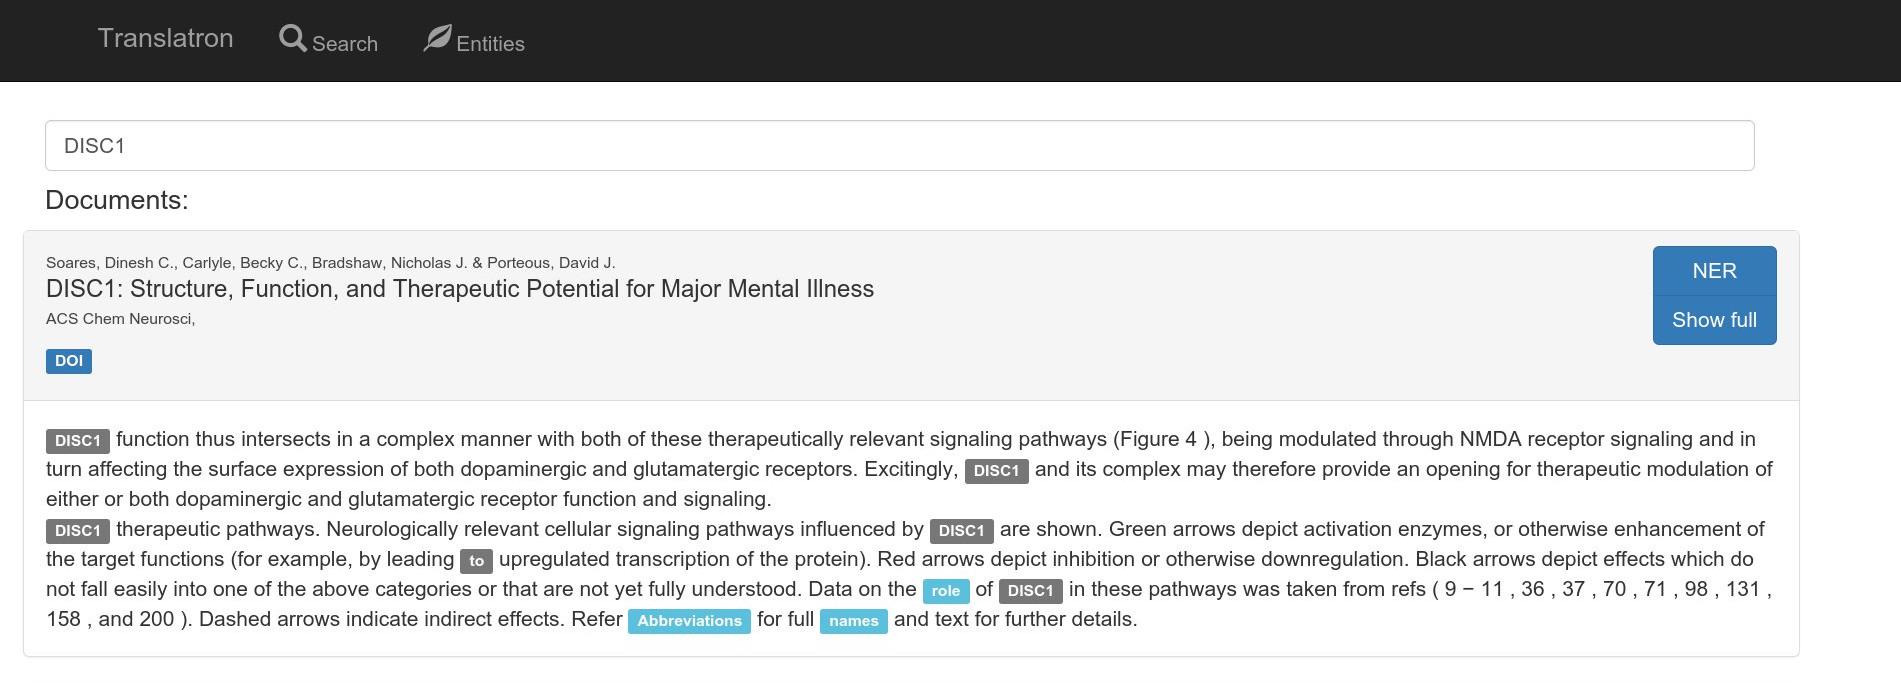
\includegraphics[width=\textwidth]{Figures/Translatron-NER.eps}
  \caption[Translatron NER example]{Translatron NER example using UniProt and MeSH as ontology}
  \label{fig:translatron-ner}
\end{figure}

In the user interface, NER hits in Translatron are marked as colored boxes, with the boxes being colored depending on the source database. In figure \ref{fig:translatron-ner}, gray hits represent UniProt hits (from other database IDs being cross-referenced in UniProt) while blue hits represent MeSH terms. Green terms would indicate UniProt IDs, \ie hits where the UniProt ID or name itself matches the text. In this example, however, no such hits have been found.

This approach allows the user to easily distinguish between different aspects of entities, as for a specific use case the coloring scheme can be fully customized: Not only can it be applied to NER hit sources but also to properties like the source taxonomy of a specific hit.

By clicking on the hits, the user is automatically redirected to a page where details about the found entity are shown. Figure \vref{fig:translatron-entities} shows the entity information that is shown when clicking on \itquote{DISC1} in figure \ref{fig:translatron-ner}. Although currently only a limited amount of information is imported and displayed for both entities and documents, it is clearly visible from figure \vref{fig:translatron-entities} that the interface concept can display a multitude of useful information to the user. Most importantly, arbitrary cross-database links such as GO terms (Gene ontology, see \cite{ashburner2000gene}) are supported (also see section \ref{ssec:limited-import-capability}).

Additionally, Translatron's ontology backend automatically imports the UniProt meta-database (see \cite{uniprot-metadb}) -- thus, hovering the mouse pointer over the name of a database display a description of said database. Additionally, for any UniProt cross-referenced database, links to the database itself and to all entries are automatically created, facilitating fully automatic cross-linking. The data imported from the meta-database can be overridden or extended by modifying a simple JSON file -- therefore providing not only the possibility to correct for errors in the UniProt meta-DB but also allowing custom databases to be added without restrictions.

\begin{figure}[!htb]
  \centering
  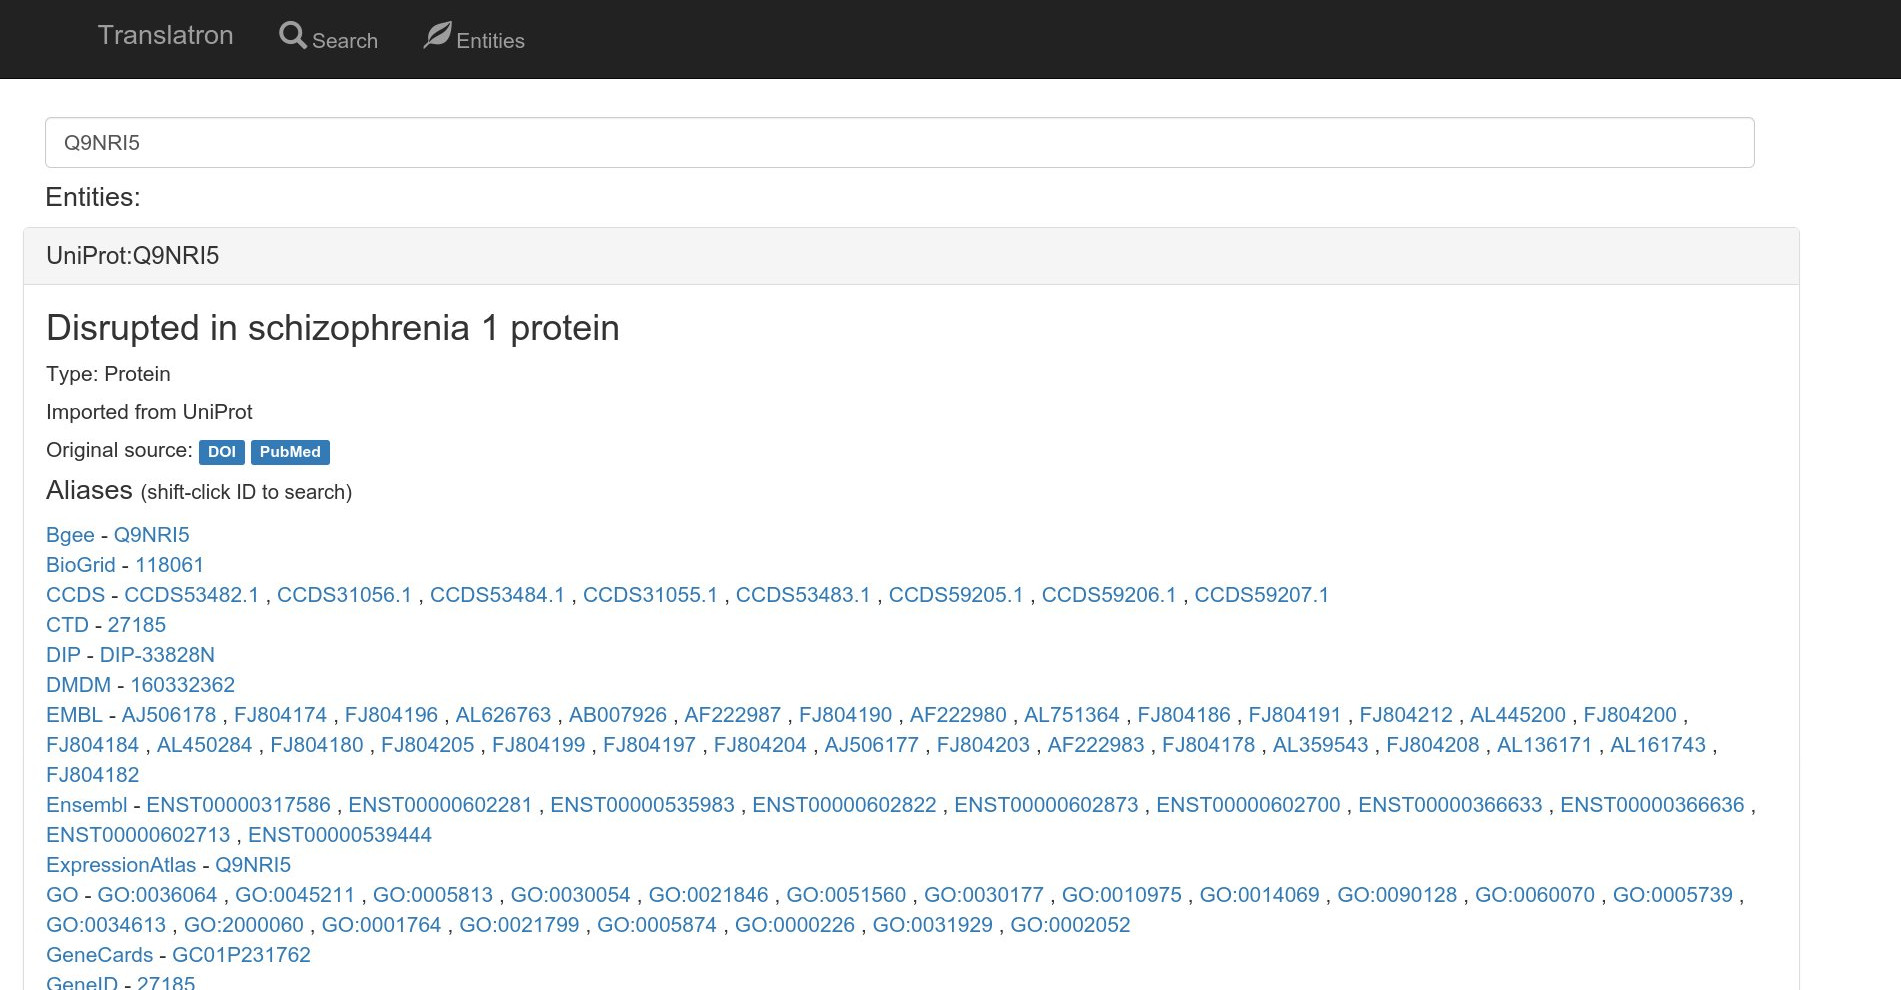
\includegraphics[width=\textwidth]{Figures/Translatron-Entity.eps}
  \caption[Translatron entity search example]{Translatron entity search example (screenshot)}
  \label{fig:translatron-entities}
\end{figure}

While search modes such as lemmatization (see section \ref{sssec:nersearchmodes}) could be implemented in Translatron, the current implementation uses case-insensitive search for the document full-text search while the NER and the entity viewer use a case-sensitive search mode. Although there are various applications where selectable and more complex search modes would be useful, this decision was made in order to provide the most simple implementation possible -- in effect facilitating easier extensibility (also see section \ref{ssec:extensibility}).

\subsubsection{Domain-specific ontologies}\label{sssec:domain-specific-ontologies}

The concept of domain-specific text corpora, as discussed in section \ref{ssec:domain-specific-textmining}, can also be applied to ontologies: When using an oversized ontology that covers more than the required domain of information, it is likely that NER hits that are considered interesting for the specific use case will be hidden by the multitude of irrelevant hits.

For example, a chemist only interested in finding chemical identifiers from inorganic chemistry would commonly not want to see protein identifiers that are present in the text. By using Translatron, it is easily possible to build a fully domain- and application-specific ontology that can also be updated on-the-fly. Based on the NER architecture and the backup feature (see section \ref{ssec:redundancy}), this ontology can also easily be exchanged without the requirement of re-indexing any document.

In order to illustrate the argument of unspecific hits hiding relevant ones, an experiment has been performed with Translatron, encompassing not only the UniProt ontology, but also Wikipedia (see \cite{wikipedia}) where every Wikipedia page title is considered an entity:

\begin{figure}[!htb]
  \centering
  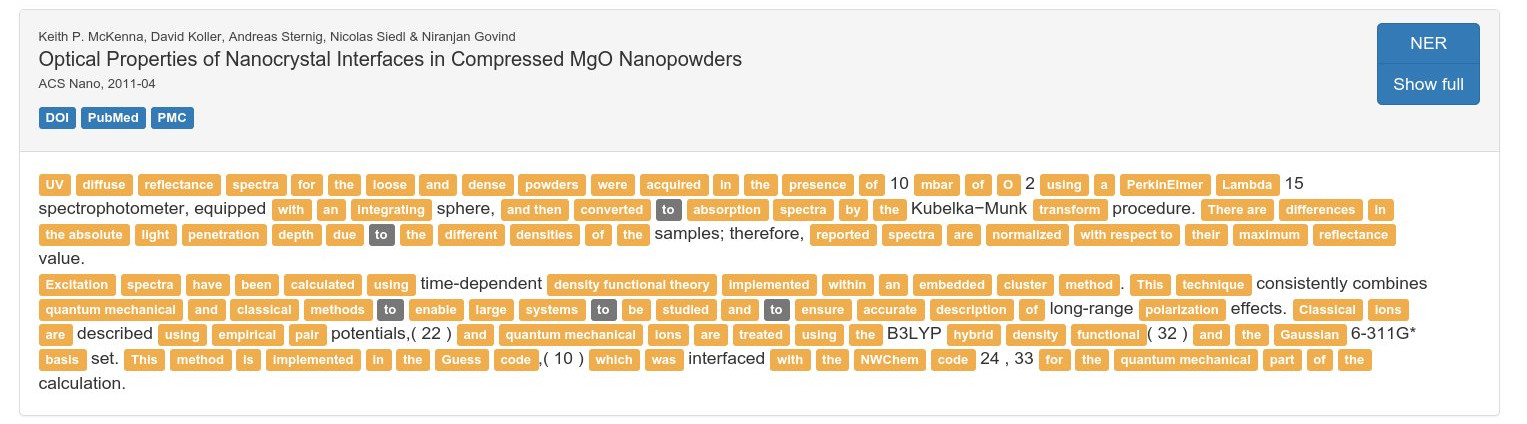
\includegraphics[width=\textwidth]{Figures/Translatron-Wikipedia.eps}
  \caption[Translatron NER with Wikipedia ontology]{Translatron NER performed with Wikipedia as ontology (screenshot)}
  \label{fig:wikipedia-ontology}
\end{figure}

As can be observed in figure \ref{fig:wikipedia-ontology}, the large amount of entities being present in the ontology leads to a cluttered result as virtually every word or word pair in the text is found as a Wikipedia hit. Although Translatron is able to provide some level of differentiation by using separate colors for different entity sources (in this example, Wikipedia is colored orange), likely the user will miss significant hits.

Using domain-specific ontologies, this behavior can be easily circumvented. Not only can the user preselect certain classes of entities to find, the operator can also dynamically add or remove entities based on the search results, facilitated by the lightweight architecture and extensibility of Translatron (also see section \ref{ssec:extensibility}). For example, the aforementioned chemist could easily remove the trivial names of noble gases from the ontology the search results are cluttered by too many hits for this class of entity. Although creating and maintaining a specific ontology requires more effort than simply importing entire databases in an unfiltered manner, it is likely that for many applications the benefit will outweigh the costs.

\section{Algorithms for resource-efficient text mining}

Although it is frequently claimed that a single algorithms will solve one problem for any possible use case, today, many designers consider the \itquote{One size fits it all} paradigm outdated (see \cite{stonebraker2005one}). Due to the inherent focus of Excerbt's algorithms on raw performance commonly disk space or main memory utilization is traded for an increased speed. Therefore it provides significant benefits for large-scale text mining applications -- however, a separate set of algorithms needs to be used to facilitate smaller-scale text mining specially fitted for resource-constrained devices.

In the following sections I will examine seven new algorithms that are implemented in Translatron to optimize its three core subsystems NER, search and user interface for resource-constrained devices.

\subsection{PRIMORDIAL indexing}\label{sec:primordial}

When using concepts like inverted indexing to index large corpora of biomedical texts, it is obvious that only a tiny fraction of the terms that are stored in the index will actually be searched. Although no authoritative statistics on this aspect seem to be available, for this thesis we will conservatively assume that 5\%\footnote{The actual number is presumed to be highly variant, but based on specific tasks performed with Excerbt this value might be less than 0.01\% for non-domain-specific or broad-domain corpora.} of the terms are actually searched for even in a heavily used system.

Assuming any entry in the index consumes the same amount of time during the indexing phase, this means that 95\% of the indexing time (irrespective of overhead) is ultimately wasted.

Unless one can accurately predict all actual search terms in advance, though, it is clear that this overhead can't be avoided entirely. Using \textit{PRIMORDIAL}, however, one can significantly reduce said overhead by using \textit{laziness} in order to perform a subset of the indexing operations not in advance for all index entries but only \itquote{on-demand}, \ie when the term is actually searched.

\begin{figure}[!htb]
  \centering
  \includegraphics[width=\textwidth]{Graphics/PRIMORDIAL.eps}
  \caption[PRIMORDIAL data flow]{PRIMORDIAL simplified data flow}
  \label{fig:primordial}
\end{figure}

\begin{figure}[!htb]
  \centering
  \includegraphics[width=0.4\textwidth]{Graphics/MergeOperators.eps}
  \caption[Merge operator overview]{A high-level overview on merge operators}
  \label{fig:merge-operators}
\end{figure}

In figure \ref{fig:primordial}, PRIMORDIAL's approach on the left is compared with classical, \itquote{eager} (as opposed to \textit{lazy}) indexing on the right. The creation of inverted indices can be simplified to -- for each token to be indexed -- building a list of documents containing that token (this mapping is symbolized by $\longrightarrow$ in the figure, with the token on the left and the entries on the right). When searching for that token, one can simply look it up in the database and thereby retrieve a list of documents containing that term.

For this example, we assume that for the token \itquote{prion}, the document \itquote{PMC:987} is already present in said list and \itquote{PMC:123} and \itquote{PMC:456} shall be appended to that list in the ongoing indexing operation.

In the classical approach, the old value will be read from the database, the new values will be appended to the list and finally the enlarged list is written back into the database. Although highly variant with the implementation, creating and writing this list for the current token many times (up to once for every single index entry) can be presumed to consume a significant amount of resources over the whole indexing run.

In PRIMORDIAL, this step works differently: Instead of performing this evaluation immediately -- we recall, in 95\% of the cases this time is wasted as the value will never be used -- PRIMORDIAL only evaluates it if and when this specific row in the database is queried, thereby saving a significant amount of indexing time (see the lower part of figure \ref{fig:primordial}). When the value is queried for the first time, the evaluated list is immediately written back into the database, yielding a virtually zero overhead solution for subsequent queries. In figure \ref{fig:primordial} unevaluated writes are symbolized by dashed boxes containing one or more entries.

One core question remains: How can this concept be implemented without requiring manual interaction from any developer extending or modifying the system?

Fortunately, YakDB provides a built-in solution: By using the mechanic of \textit{merge operators}, one can define an arbitrary function to merge two or more distinct writes into a single binary value. In figure \ref{fig:merge-operators} an example of the execution of a simple merge operator is shown: It operates on two values \itquote{value1} and \itquote{value2}, producing \itquote{value1value2} by simple appending the last input to the first.

The merge operators in YakDB are evaluated only (in the scope of a single key) if at least one of the following criteria is met:
\begin{itemize}
 \item The key is queried or a sequential scan is performed that includes the key
 \item Certain database-level automatic partial compactions occur whose discussion would exceed the scope of this thesis
 \item A full or partial compaction is manually requested
\end{itemize}

Particularly interesting for some use cases is the last option: If an application requires maximum search speed even for the first time when a key is read or if the space overhead of PRIMORDIAL is not considered acceptable, it is possible to perform a database-level compaction. This operation can either be performed on a specific key range or on the whole database, in effect evaluating all keys and storing them as space-efficient as possible without sacrificing performance. Although heavily variant and therefore hard to benchmark, compaction takes about five minutes per gigabyte database size (measured before compaction) on modern computers.

% Even if the option of full evaluation by compaction is chosen, the indexing process appears faster as the database will not consume much CPU time for evaluation during indexing. Additionally, when compared to most existing databases, the indexing process is more efficient. In early versions of Translatron, the YakDB implementation of the PRAISER merge operator only allowed merging two values at once. This resulted in the inefficient evaluation of large list merges as very common GO terms were associated with millions of UniProt entries. Therefore, the indexing of UniProt entities took several hours -- with the new, improved merge operator implementation this could be reduced to only a few minutes. However, it is assumed that many existing databases like PostgreSQL will only support the inefficient eager evaluation as they are not capable of performing lazy evaluation by design -- in effect, creating and writing a new list even if that list grows to millions of entries.

Note that PRIMORDIAL by itself does not specify a particular merge operator, making its core approach also applicable to other applications. Furthermore, the index structure itself is only handled in an abstract manner by PRIMORDIAL: Beyond simple lists of occurrences, the core algorithm also supports more complex structures like hierarchies, graphs or spatial trees -- the semantic that is supported only depends on the merge operator implementation in use. This also means that PRIMORDIAL itself does not handle concepts like incremental indexing but leaves it to the merge operator implementation to provide guarantees about its behavior.

\clearpage

%%%%%%%%%%%%%%%%%%%%%%%%%%%%%%%%%%%%%%%%%%%%%%%%%%%%%%%%%%%%%%%%%%%%%%%%%%%%%%%%%%%%%%%%%%%%%

\subsection{PRAISER merge operator}\label{sec:praiser}

In contrast to Excerbt, Translatron can be used as a highly dynamic system: Not only can a domain-specific corpus and ontology be used, but those can also be modified on demand. While removing and modifying individual documents is also supported yet not implemented, it inherently requires a full reindexing run with an anteceding index truncation\footnote{In this context, truncating means emptying the respective table.}, therefore not exhibiting any specific issues.

Referring to the basic workflow depicted in figure \vref{fig:import-workflow}, incrementally adding documents poses a potential problem because the re-indexing that needs to be performed does not provide intrinsic guarantees about adding duplicate results to the inverted index.

It is obvious that users don't want to see those identical duplicates in a list of search results -- they only provide redundancy without any added information. However, algorithms simply removing duplicates might introduce \textit{instability}, meaning that the order of the search results will be changed completely even if only a single new search result has been added. Although it is arguable if stability is required for practical use cases, very large lists of search results are not expected to look totally different when adding only a single document.

This is where PRAISER comes in: It provides a simple PRIMORDIAL-compatible merge operator that not only provides guaranteed removal of redundant elements but an inherently stable, lexicographical sort order.

\begin{figure}[!htb]
  \centering
  \includegraphics[width=0.3\textwidth]{Graphics/PRAISER.eps}
  \caption{PRAISER schematic}
  \label{fig:praiser}
\end{figure}

As shown in figure \ref{fig:praiser} PRAISER consists of two simple steps that are performed on the result list when the merge operator result is evaluated (see \ref{sec:primordial} on lazy evaluation):
\begin{enumerate}[label={(\arabic*)}]
 \item \textbf{Place all elements into a set}: This removes redundancy but might scramble the ordering
 \item \textbf{Sort by binary lexicographic ordering}, restoring a guaranteed sorted order without any assumption about the elements themselves
\end{enumerate}

By using special ordered sets like binary tree sets, the set itself will perform step (2), eliminating intermediary results and overhead.

As YakDB currently only provides a predefined set of merge operators that, besides merging, also need to handle binary (de)serialization, the so-called \itquote{NUL-separated set append} operator has been implemented in YakDB, using aforementioned ordered set implementation with list elements separated by NUL characters.

%\afterpage{\clearpage}

%%%%%%%%%%%%%%%%%%%%%%%%%%%%%%%%%%%%%%%%%%%%%%%%%%%%%%%%%%%%%%%%%%%%%%%%%%%%%%%%%%%%%%%%%%%%%%%%%%%%%%%

\subsection{PERSIST single token indices}\label{sec:persist}

One of the main reasons why inverted indices consume large amounts of disk space is the support for multi-token searches. Intuitively, users expect from a full-text search engine not only proper results when searching for \itquote{prion} but also when querying for \itquote{prion disease}.

Assuming that the expected search result are documents where in some context\footnote{Examples for this context would be the paragraph, the sentence, within two words of each other or even the entire document.} the terms \itquote{prion} and \itquote{disease} appear together, the algorithm performing the search must implement a way to filter out all hits where this condition is not fulfilled.

One classical solution for this issue is to not only index single terms, but also any $k$-permutations of tokens that occur in the text. What value of $k$, \ie the maximum number of tokens that are indexed together, is chosen, depends on the usage scenario. This approach has the core advantage that for most use cases one query only requires a single database lookup.

The formula for the number of $k$-permutations, assuming $n$ tokens with $k \leq n$ in the context and is well-known:

\begin{align}\label{eq:permutations}
 P_k(n) &= \frac{n!}{(n-k)!}
\end{align}

From equation \eqref{eq:permutations} it trivially follows that when indexing all $2{\dots}k$ tokens the number of index entries\footnote{Note that an entry in this context is not necessarily a distinct key in the index database but rather one element in the list of references for a potentially pre-existing key in the index.} is defined as:

\begin{align}\label{eq:permutations2}
 P_{2{\dots}k}(n) &= \sum_{h = 2}^{k}\frac{n!}{(n-h)!}
\end{align}

Assuming $n = 20$ and $k = 5$, a single sentence will generate \num{1983980} entries according to equation \eqref{eq:permutations2} -- an almost \num{100000}-fold overhead when compared to the $n = 20$ single tokens that need to be indexed for single-token-only search. While in practice this number can be reduced by marking a significant fraction of those permutations as redundant or irrelevant (\eg stopwords which are generally not indexed), the amount of overhead that remains makes this algorithm unusable for space-constrained devices. 

PERSIST provides a space-overhead-free alternative to the aforementioned approach. It indexes only single tokens and computes multi-token queries by using set intersections of single token results, using the following procedure:
\begin{enumerate}[label={(\arabic*)}]
 \item Split the search query into a set of tokens (\itquote{query tokens}) using the preconfigured tokenization function
 
 \item Remove stopwords from the query tokens. Stopwords are guaranteed not to generate any result if the index has been built properly.
 
 \item Fetch single-token search results for all query tokens
 
 \item Compute the set intersection of all fetched search results. Optionally, skip search result sets that would result in an empty result. This is a simple case of automatically correcting the query as it is likely that the user does not intend seeing an empty result. The YakDB / Translatron stack implements this option -- however, the user is currently not notified if a query token is ignored due to this feature.
 
 \item (Optional) Filter out search results where the search terms are present in the wrong order by checking the original context. This step is not currently implemented by Translatron which thereby increases the rate of false positives, but also exhibits a lower false negative rate. As a default configuration, this is considered advisable as the user will likely tolerate irrelevant search results if potential true-positive results the operator is looking for are shown in the result list.

\end{enumerate}

Obviously, this step yields the correct result set because a result appears in the final result set exactly if it appears in all of the single-token search results. For example, in the sentence
\begin{quote}
 \itquote{$PrP^{Sc}$ causes ovine prion diseases}
\end{quote}
when searching for \itquote{prion diseases} in the sentence context, the sentence will appear on the result list because it appears on both the single-token search result for \itquote{prion} and the one for \itquote{diseases}.

During this step, however, the function used to determine equality of two results is critical as it determines the search context. For example, in Translatron, a paragraph context is assumed by default (\ie a search result is considered a hit if all tokens are found in the same paragraph). Therefore, Translatron uses a binary format for elements of the inverted index that contains both the document identifier and the paragraph number. Therefore, a simple binary equivalence function can be used during the set intersection as this configuration intrinsically checks for equivalence of both the document identifier and the paragraph number.

This issue gets more complex if the context is, for example, defined as \itquote{all tokens occur within 5 words of each other}. Depending on details regarding the definition of \textit{within 5 words of each other}, PERSIST might need to be extended so it can understand the context beyond a simple stateless set intersection. A detailed discussion, however, is considered to be highly dependent on the use case and therefore does not fit within the scope of this thesis.

Although PERSIST trades speed for space and it therefore is perfectly suited for space-constrained devices, it is doubtable whether the classical algorithm directly indexing multi-token permutations actually exhibits better performance for a practical average query: While the number of database fetches is clearly reduced, the database grows so large that the likelihood of cache hits (\ie the probability that a requested data block can be served from main memory instead of the slow disks) reduces to practically zero when assuming random lookup key. There are also multiple other reasons why most databases exhibit performance losses when the database itself grows larger that go beyond the scope of this thesis.

One possible performance issue of the PERSIST algorithm is that large text corpora may lead to the computation of multi-billion-element set intersections if the first query token is very common and not a stopword. This would significantly reduce the speed of the algorithm. The likelihood for this scenario is reduced by both the focus on smaller domain-specific corpora and the careful crafting of stopword lists.

Should this behavior be an issue in any practical use case, there is a simple solution: PERSIST can be extended to search pairs or triples of tokens if one of the tokens is very common in the corpus being used, in effect creating a combination of PERSIST and the classical solution. This significantly reduces the set size -- however, an implementation is likely to be more complex and trades space consumption for speed, with a speedup possibly being only observed for a small subset of the queries.

\afterpage{\clearpage}

%%%%%%%%%%%%%%%%%%%%%%%%%%%%%%%%%%%%%%%%%%%%%%%%%%%%%%%%%%%%%%%%%%%%%%%%%%%%%%%%%%%%%%%%%%%

\subsection{PRESIDE prefix search}\label{sec:preside}

When using a search engine that supports real-time queries (\ie the search is performed while the user is typing) it can easily be shown that simple exact searches in an inverted index are likely to generate unintuitive search results:

Consider, for example, the query \itquote{prion}. In a real-time-capable full-text search engine\footnote{\ie a search engine that generates a query for every typed character.} using simple case-insensitive search and with a corpus containing only the sentence
\begin{quote}
 \itquote{$PrP^{Sc}$ causes ovine prion diseases}
\end{quote}
the following query-result pairs are generated:

\begin{itemize}
 \item p - No results
 \item pr - No results
 \item pri - No results
 \item prio - No results
 \item prion - Aforementioned sentence is shown as result
\end{itemize}

However, clearly the expected behavior is to see the aforementioned sentence as a search result (which can be considered a best-match) for any of those queries.

The simplest yet obvious solution is to use prefix search: All of the queries without any result are intrinsically prefixes of the full query \textit{prion}.

However, prefix search is hard to implement in a performance and space-efficient way using conventional databases. YakDB, though, provides the built-in scan mechanism that allows efficient iteration over database entries in lexicographical order -- PRESIDE is the application of this method for prefix full-text search.

For the query (and therefore prefix) \itquote{pri}, database entries like \textit{print}, \textit{primal} and \textit{primary} can be found. As a stop key\footnote{\ie the first key that will not be iterated over.} for the scan operation, \textit{prj} can be used: Any entry which is prefixed by \textit{pri} is guaranteed to be less than \textit{prj} in lexicographical order. Furthermore, any arbitrary entry that is not prefixed by \textit{pri} is either less than \textit{pri} or greater than or equal to \textit{prj}, yielding intrinsically correct results.

However, the user must take special care that not too many results are selected by the scan operation. For instance, the query \textit{p} would select all entries starting with \textit{p} -- for a large corpus, this might yield many millions of result entries. Therefore, PRESIDE is parameterized with a maximum number of database entries it will iterate over (whichever event happens first, the scan limit or the stop key being reached, will stop the iteration). This approach in effect allows limiting the resources consumed by a single scan request.

When being used in conjunction with PERSIST (see section \ref{sec:persist}), PRESIDE requires a scan for every single query token of a multi-token query. Although this intrinsically reduces the performance\footnote{Not only because scans are intrinsically slower than single reads but also because multiple reads can be joint into a single YakDB request while multiple scans can not.}, scans are generally considered a fast operation in YakDB and the improved query flexibility seems to be worth the extra CPU time spent even for slower setups.

In its default configuration, Translatron generally searches for prefixes when querying the document database, while entities are searching by exact match -- this behavior is easily adjustable, though. Because of the intrinsic properties of PRESIDE, both types are supported with the same index and do not require any database modification.

%%%%%%%%%%%%%%%%%%%%%%%%%%%%%%%%%%%%%%%%%%%%%%%%%%%%%%%%%%%%%%%%%%%%%%%%%%%%%%%%%%%%%%%%%%%%%%%%%%%%%%%

\subsection{PRO-PANE result ordering}\label{sec:pro-pane}

\begin{figure}[!htb]
  \centering
  \includegraphics[width=0.8\textwidth]{Graphics/PRO-PANE.eps}
  \caption{PRO-PANE example schematic}
  \label{fig:pro-pane}
\end{figure}

For Google -- one of the most-used generic search engines available today -- one of the biggest factors for success is to increase the relevance and thereby the perceived quality of the search results (see \eg \cite{pant2000computer}). As already discussed in section \ref{sec:preside} and section \ref{sec:persist}, for Translatron it is therefore relevant to generate search results that match the user's expectation. Although it is likely that with a simple system one can't achieve the level of search customization and adaptivity that Google provides for the generic use case, very simple optimizations can lead to a significant improve in search result quality.

One of the most important aspects of relevance is the order of search results -- in other words, the displaying of more relevant result before less important ones. However, without focusing on a very specific use case, it is hard to define relevance in this context. PRO-PANE is a generic search result reordering algorithm that circumvents this intrinsic problem by allowing an arbitrary number of \textit{relevance classes} with an programmable order relation on said classes that can be changed for each individual query. By using PRO-PANE, this simple concept can be stored efficiently in key-value databases.

As depicted in figure \ref{fig:pro-pane}, PRO-PANE hooks into the indexing phase by prepending the relevance class to the key. In most use cases (including the default configuration of Translatron), these relevance classes are equivalent to the coarse location of the hit. For instance, Translatron defines the three relevance classes \texttt{title}, \texttt{text} and \texttt{meta} -- this is based on the assumption that when a user searches for an arbitrary term, the expected result is to see hits from a document's title before hits from the full text or even hits from the metadata.

PRO-PANE consists of three core hooks\footnote{A hook is a part of a program that is injected into an existing process and modifies its behavior.}:
\begin{itemize}
 \item An indexing hook that extracts the relevance class from the hit and prepends said relevance class.
 \item A lookup hook that modifies the query database lookup (see section \ref{sec:persist} for details): The database read requests are modified so that for each query token all relevance classes are queried. For performance-critical applications, it is possible to query only a subset of the relevance classes for specific queries.
 \item A sort hook that sorts the result after lookup and filtering. This uses the order relation defined on the relevance classes to, for example, select \texttt{title}-class hits before \texttt{text}-class hits.
\end{itemize}

When the overall number of hits should be limited, PRO-PANE uses a parameterized selection scheme that iterates over the relevance class hit lists and builds a result list:
\begin{itemize}
 \item Initialize the result list $r$ to be empty
 \item Loop over the relevance classes, highest relevance first:
 \begin{itemize}
  \item Append all hits from the current relevance class to $r$
  \item If the length of $r$ is less than the \textit{minimum hits} parameter, continue with the next relevance class (if any)
 \end{itemize}
 \item If the length of $r$ is greater than the \textit{maximum hits} parameter, remove everything except the first \textit{maximum hits} entries from $r$
\end{itemize}

Assuming \textit{maximum hits} $\geq$ \textit{minimum hits}, this algorithm ensures that a) no more than \textit{maximum hits} are present in any case and b) if a certain number of hits (\textit{minimum hits}) is reached by using only results from high-relevance classes, no results from lower-relevance. A common configuration is to set \textit{minimum hits} $=$ \textit{maximum hits}, which is equivalent to taking the first \textit{maximum hits} elements from a concatenated list of all relevance classes.

By default, Translatron uses \textit{minimum hits} $ = 50$ and \textit{maximum hits} $ = 250$. However, these parameters are generally expected to be variable with the specific use case.

%%%%%%%%%%%%%%%%%%%%%%%%%%%%%%%%%%%%%%%%

\subsection{FiT-NESS multi-token NER}\label{sec:fitness}

\begin{boxedDefinition}[Single-/multi-token entity identifier]\label{def:singlemultitokenentity}
A single-token entity identifier is defined as a nonempty entity name which, when processed with a given tokenization function, yields a token list having a length of one.\\\\
A multi-token entity identifier is defined as any identifier for which the criteria for a single-token identifier do not apply.
\end{boxedDefinition}


\begin{figure}[!htb]
  \centering
  \includegraphics[width=0.5\textwidth]{Graphics/FITNESS.eps}
  \caption[FiT-NESS NER example]{FiT-NESS named entity recognition example}
  \label{fig:fit-ness}
\end{figure}

In practical NER implementations, there are significant differences between indexing and search for single-token entity identifiers (see definition \ref{def:singlemultitokenentity}) as compared to NER algorithms that also support multi-token entities\footnote{Although single-token identifiers can be seen as special cases of multi-token identifiers, it is often advisable to handle them differently due to the increased overhead of multi-token identifier processing.}.

For example, similar to single- and multi-token queries (see section \ref{sec:persist}), a multi-token capable NER not only has to be able to find an occurrence of \itquote{prion} but also an occurrence of \itquote{prion diseases}.

When using a \textit{percolator}-type NER like Excerbt or Translatron (see \cite[section 4.3.1]{wachinger2013next} and the discussion in section \ref{sssec:ner-excerbt-translatron}), though, one has to deal with a major issue which is most relevant for space-constrained devices:

When indexing the entity \itquote{prion diseases}, the entity yields two index entries, one for \textit{prion} and one for \textit{diseases}. The number of entries can also be defined as:
\begin{align}\label{eq:index-num-tokens}
\begin{split}
E(n) &\in \mathcal{O}(n)\\
\text{where~} E(n) &= \text{Number of index entries for an entity containing $n$ tokens}
\end{split}
\end{align}
This property is most relevant for entities containing many tokens like IUPAC identifiers (if splitted by dashes), as these will fill up the index with a significant number of entries.

FiT-NESS, however, approaches the NER problem differently: Instead of indexing every single token of a multi-token entity, it only indexes the first token, thereby achieving $E(n) \in \mathcal{O}(1)$ space complexity and finds multi-token hits via postprocessing. As a side effect, the internals of this algorithm are also regarded to be significantly more simple than a full implementation of a classical multi-token NER.

As shown in figure \ref{fig:fit-ness} the core algorithm consists of three core phases:
\begin{itemize}
 \item Indexing, where only the first token of an entity (\eg \textit{prion}) is stored in the inverted index with a reference containing the full identifier of the entity (\eg \textit{prion diseases})
 
 \item Search, where every token contained in the text is looked up in the database. Duplicate tokens in the document can be skipped during the lookup. Using the YakDB feature of multi-key read requests, an entire document generates only a single request to the database using this approach.
 
 \item Postprocessing, where for any hit of a first token the implementation checks if the subsequent tokens in the document match the subsequent tokens in the original entity identifier. This step needs to be performed for every occurrence of the first token in the document. If all tokens match, the location in the document is considered a NER hit.
\end{itemize}

Obviously, FiT-NESS does not require a separate implementation for single tokens as the postprocessing phase will always yield a hit if no subsequent tokens are present in the entity. This reduces the overall complexity of the code.

In its current form, FiT-NESS does not implement fuzzy search. For instance, it would not find an instance of the entity \textit{prion diseases} in the text \itquote{prion-transmitted diseases}. However, the algorithm is easy to modify, for example by searching for the next token in the same sentence instead of expecting a match in the next token -- this can be done performantly by, for example, using a modified version of the Boyer-Moore algorithm operating on words instead of characters (see \cite{boyer1977fast}). Even a definition of fuzziness where no exact match for the first token is required can be implemented, albeit this is significantly more difficult: One can also index one or more tokens besides the first one, creating a combination of FiT-NESS with the classical algorithm.

FiT-NESS -- as implemented in Translatron -- might exhibit slight performance issues if the first token of an entity is very common and thus, the inverted index entry for said first token grows very large. However, this case is presumed to be unlikely for Translatron's use case, especially if domain-specific ontologies as discussed in section \ref{sssec:domain-specific-ontologies} are used.

\afterpage{\clearpage}

%%%%%%%%%%%%%%%%%%%%%%%%%%%%%%%%%%%%%%%%%%%%%%%%%%%%%%%%%%

\subsection{WESTSIDE client interface}\label{sec:westside}

In contrast to the other six algorithms that have been discussed in this chapter, WESTSIDE does not improve processes that are internal to the server but the client-server communication strategy.

Most web-based systems use the HTTP protocol in order to communicate with the server. However, in the context of text mining systems this leads to five major issues:
\begin{itemize}
 \item \textbf{Connection overhead}: With HTTP, every client-server communication has not only overhead generated by parsing comparatively large HTTP headers but also overhead due to the setup of a new TCP connection. Although mechanisms like the HTTP Keep-Alive header (see \cite{nielsen1997network}) are widely deployed to alleviate the impact of those issues, it is difficult to avoid this overhead altogether, in effect leading to increased latency and lower throughput, both of which are relevant for real-time search under certain circumstances.
 
 \item \textbf{Stateful client connections require additional layers}: HTTP by itself does not group requests by client. Although this feature can be implemented with cookies and similar pseudo-stateful methods, it is hardly possible to associate information to a client without adding a significant amount of complexity to the server software -- therefore, if no complex session layer must be used, the server can only use stateless client connectivity.
 
 \item \textbf{Asynchronous database connections}: If it is not possible to associate a dedicated database connection to a client due to statelessness, one global connection (or a pool of connections) has to be used. Although the semantics of those connections vary significantly from database to database, most connections either perform locking and therefore degrade the system performance or require the developer to manually re-associate responses to their original requests like YakDB: Those asynchronous database connections add a significant amount of complexity to the system, thereby limiting its extensibility.
 
 \item \textbf{Unordered client requests}: Even if mechanisms like keepalive are used, there is no guarantee that client requests arrive in the same order they were sent in. Stateful algorithms extending Translatron's client/server communication might, however, might depend on a specific order of messages.
 
 \item \textbf{Communication can only be initiated by the client}: The server is not able to send a message to the client without the client first sending a request to the server. Commonly, this issue is circumvented by using mechanisms like \textit{long polling} (see \cite{loreto2011known}) -- however, this introduces extra overhead and does not allow true bidirectional communication.
 
\end{itemize}

In order to resolve these issues, a protocol called WebSocket was standardized (see \cite{fette2011websocket}, \cite{hickson2011websocket} and \cite{rfc6955}) that uses HTTP only for protocol negotiation and then falls back to a message-based communication scheme featuring true bidirectional communication.

By using a single WebSocket connection per client, WESTSIDE is able to resolve all the aforementioned issues. Not only can a single database connection be associated to a single client in a stateful manner, WebSockets also provides guaranteed ordering of messages, decreasing the likelihood of complex failure modes for both the client and the server.

For example, in earlier versions of Translatron there was an issue with real-time search (also see \ref{sec:preside}): When the user typed the first characters, the queries were very short and therefore produced a large number of results, significantly increasing the time required to process the query. When refining the query, however, the query processing intrinsically got faster as the number of results decreased. However, the user interface was configured to replace the displayed search results with the new ones whenever a response arrived at the client. When typing sufficiently fast, though, processing the shortest query took longer than processing the longest, most specific one -- leading to one of the shortest queries to arrive last at the client. Therefore, after the user finished typing the last character of the search term, frequently an earlier, less specific request arrived as the last response. This caused the user interface to render, for example, the result for the \textit{pr} query when the user actually typed \textit{prion}.

This is a prime example of a complex failure mode that only occurs under very special circumstances like a certain database size, a certain CPU speed, certain dynamic cache characteristic etc. and is therefore hard to anticipate if the system is not intrinsically safe against a particular class of issues.

WebSockets, on the other hand, allow implicit sequentialization of requests -- in other words, the server will strictly process one request after the other and therefore will also respond in the correct order. Additionally, WebSockets are virtually overhead-free\footnote{Although WebSocket messages require a header and in the client-to-server direction also requires a special encoding (see \cite{rfc6955}), these factors have little contribution to the actual amount of CPU time consumed on modern computers.} without sacrificing the simplicity of Translatron's design.

In the current version of Translatron, the WebSocket communication is handled on port 9000, in separate to the HTTP server that serves the static user interface. This behavior might cause issues with firewalls that don't allow port 9000 to pass through. As Translatron is built primarily to run on the local computer or in the local network, this is not generally considered an issue.

\afterpage{\clearpage}

%%%%%%%%%%%%%%%%%%%%%%%%%%%%%%%%%%%%%%%%%%%%%%%%%%%%%%%%%%%%%%%%%%%%%%%%%%%%%%%%%%%%%%

\chapter{Summary \& Outlook}

In this thesis, concepts and algorithms facilitating domain-specific text mining on resource-constrained devices have been discussed.
The proof-of-concept tool Translatron provides an implementation of many novel algorithms and concepts that have been analyzed -- in conjunction with the bioinformatics-focused YakDB database, this approach provides a high-performance scaffold on which customized text mining applications can be implemented.

Due to the focus on resource-constrained devices and a domain-specific approach, Translatron can be used to facilitate text mining where before this was impossible: Existing tools generally require powerful servers or clusters that are hard to maintain and fail more frequently than a local mining tool like Translatron.

\section{Limitations of Translatron}\label{sec:limitations}

Although it has been shown that Translatron has inherent advantages when compared to systems like Excerbt, it does not represent a finished, ready-to-use system: Its proof-of-concept nature also connotes that it is not expected to be bug-free -- without modification is likely unsuited for most use cases.

It is therefore important to discuss not only limitations and potential shortcomings of the current Translatron version, but also possible solutions for these issues.

Due to the complex nature of the text mining topic, this list can't be exhaustive -- instead, the most important points that have not been discussed yet in chapter \ref{chapter:translatron} are outlined so future users of Translatron can easily find their way around its drawbacks.

\subsection{Missing semantic features}\label{ssec:missing-semantic-features}

In contrast to Excerbt, Translatron is not a full-featured relation extraction engine but a full-text search engine with an integrated ontology. Although this means Translatron's architecture is more simple and lightweight, applications like Negatome 2.0 (see \cite{blohm2013negatome}) that depend on the relation feature of Excerbt are not possible without adding a complete SRL stack to Translatron.

Representing Excerbt's relation graph in YakDB is easy due to the built-in graph library. However, as discussed by Wachinger in \cite{wachinger2013next} SRL-based systems still have significant issues understanding natural language. For example, they have issues determining the meaning of cross-sentence relations and natural ambiguities in the language in use that can only be resolved by a person having a deep understanding of the context. This area is actively researched, however, and might profit from the easy extensibility of Translatron. Without writing an entirely new text mining system for every new NLP algorithm, a researcher could use Translatron as a basis for the evaluation of new algorithms.

\subsection{Cluster use of Translatron}\label{limitations:clustering}
 
As discussed in section \ref{ssec:clustering}, the Translatron/YakDB stack by itself do not support clustering -- though, with YakDB's distributed data processing as examined in section \ref{ssec:mapreduce} it would be possible to distribute, for example, semantic role labelling among multiple nodes.

Besides simple distributed computation, a distributed and therefore scalable storage can be realized by simply placing the YakDB storage directory on a clustered file system like \textit{Ceph} (see \cite{weil2006ceph}) -- even using the HDFS virtual file system driver on top of a Hadoop cluster is possible using this strategy.

One exotic and therefore rarely mentioned use of clusters that fits well into the domain-specific model is the parallel deployment of multiple instances: A single central deployment is likely not adapted to the differing requirements of different work groups and therefore inflexible at best and dysfunctional at worst. By instead deploying a high number of very lightweight, parallel instances of a software, not only is there redundancy in terms of backup instances in case one should fail, but any workgroup has the flexibility of trying out different configurations or datasets and comparing them directly. When using a cluster sized similarly to the one used by Excerbt, it is presumed that more than \num{1000} instances of Translatron could be ran in parallel, even though no authoritative tests have been performed. A single YakDB instance can easily handle multiple Translatron instances in parallel -- it is actually possible to run several Translatron instances accessing the same set of database tables and perform load-balancing using this configuration.

\subsection{Lower memory thresholds}\label{ssec:lower-memory-thresholds}

Even if Translatron is generally optimized to consume minimal amounts of both main memory and disk space, there are several reasons why Translatron can't consume an arbitrarily low amount of memory, even if using very small corpora and ontologies:
\begin{itemize}
 \item \textbf{Python interpreter}: The interpreter itself plus the Translatron Python scripts consume at most a few tens of megabytes, depending on the configuration in use. Additionally, both Translatron's source code including libraries and the Python interpreter itself require disk space in the magnitude of multiple tens of megabytes. However, a specific application requiring ultra-low disk-space utilization can replace many of the libraries by more compact, application-specific versions only supporting a minimum feature set.
 
 \item \textbf{YakDB}: Although written in \CC, the different parts of YakDB still consume between about five and multiple hundreds of megabytes of main memory, depending on the configuration being optimized for speed or for low space consumption.
 
 \item \textbf{\ZMQ\ queueing}: The queueing as discussed in section \ref{ssec:asynchronicity} consumes more memory if the queue size is set to a large number of messages and the queue is filled up. Additionally, it depends on the size of a request, as a \ZMQ\ queue always stores up to a constant number of messages and not up to a constant number of bytes. This aspect is likely to only cause transient peaks of memory consumption during high-load phases -- one example for such a scenario would be programmatic usage of the NER API that generates large read requests as discussed in section \ref{sec:fitness}.
 
 \item \textbf{Browser}: If the client also runs on a resource-constrained device, it is likely that the browser consumes a majority of the memory: Even though mobile browsers are optimized for low memory consumption, complex real-time user interfaces like the one used by Translatron will lead to an increased memory consumption, especially if multiple hundreds of results are displayed. The actual memory consumption varies heavily with the device and browser characteristics and can thus not be estimated accurately.
\end{itemize}

In general, those inherent limitations -- proper configuration presumed -- are very low and therefore should only rarely have an impact even for devices with as low as 256 MiB of main memory, provided that the browser is sufficiently efficient in terms of main memory utilization. However, it is clear that using the current architecture, Translatron can't be easily implemented on fully embedded platforms like microcontrollers (\eg for implementing the \itquote{Internet of Things} paradigm) that contain main memory in the order of hundreds of kilobytes (see \eg\hspace{-.2em}\cite{stm32f407}). This is, however, not only considered a niche application but also a class of platforms that requires yet another set of highly specialized algorithms -- therefore, analyzing this problem in detail would by far exceed the scope of this thesis.

\subsection{Lack of configurability}\label{ssec:lack-of-configurability}

In its current form, as shown in figure \vref{fig:translatron-search} Translatron is a simple full-text search engine without the possibility of adding additional filters to the search result. This shortcoming is not inherent to Translatron's design but based on the assumption that software without a large amount of features is easier to understand and therefore easier to extend -- still, it is likely that many practical applications will require a certain set of filters to improve the perceived quality of the search results.

One major limitation is the user interface: While the simple search interface is sufficient to show that Translatron's  concepts work, developing an user interface optimized for user-friendliness is beyond the scope of this thesis. Although Translatron's interface is built on a responsive basis so handheld devices are supported, rendering the search results is slow on mobile devices. Furthermore, the display of search results (both documents and entities) has not been optimized for mobile use especially on smartphones.

However, Translatron's interface is much easier to modify than, for example, Excerbt's web-based UI. For Excerbt, parts of the interface are dynamically generated by the server (therefore modifying the complex server code is required for many modifications) whereas Translatron uses a purely static webinterface consisting only of a number of files that are sent to the client without modification (also see section \ref{sec:translatron-architecture}).

In order to support features like faceted search (see \cite{koren2008personalized}), both Translatron's server and the user interface will need to be extended. For example, the user should be able to select the search mode (\eg case-sensitive or case-insensitive) and a range of years to filter the search results. Additionally, it might be advisable for some applications to manually select exact search over prefix search (also see section \ref{sec:preside}).

\subsection{Limited import capability}\label{ssec:limited-import-capability}

As depicted in figure \vref{fig:import-workflow}, Translatron currently only supports importing PMC documents and entities from UniProt, MeSH and Wikipedia. For most practical applications, this list will need to be extended significantly: For example, a microbiological application might require importing MEDLINE abstracts (a dataset which was not available during Translatron's development), PDF reports and HTML-based views of closed-access subscription papers, supplemented by metadata fetched via the OAI-PMH method (see \cite{sompel2004resource}). On the ontology side, this application might, for instance, require indexing the NCBI taxonomy, KEGG pathways and PubChem compounds.

Not only is Translatron currently limited in the number of importers it supports, but also the importers do not import and index all relevant parts of the documents. While it can be argued that not importing the amino acid sequence of UniProt entities is irrelevant, the PMC importer does not handle abstracts separately from the main text. Furthermore, PMC metadata is currently imported but not indexed, emphasizing its proof-of-concept nature.

Furthermore, not the entire set of PMC XML document can be parsed correctly by the importer: For single documents that are slightly different in format than others (for example, they might be missing an optional tag), the parser might print an error message and ignore this document. During the development of Excerbt, a similar problem was encountered: Many import formats slightly changed over time, therefore the importer required constant maintenance and testing with updated datasets. As Translatron's importers are written in Python and not optimized for speed but for simplicity, they can be modified more easily -- therefore reducing the effort required for updates and maintenance.

While those shortcomings are typical for a proof-of-concept tool and require further tests, it is clear that any productive use of Translatron will require further development and, most importantly, testing.

\subsection{Limited reindexing support}

As already discussed briefly in section \ref{sec:praiser}, the PRAISER merge operator is only designed for incrementally adding documents. Updating documents or removing them will result in false hits being present in the index as removing individual hits is currently unsupported.

Moreover, when incrementally adding documents, reindexing is not performed automatically. This means that after inserting a new set of documents, the user manually has to start the indexer. Without doing this, the new documents will not be found via the document search. This behavior is, however, not caused by conceptual shortcomings of Translatron but by implementation details. In a productive environment it might be reasonable to automatically start indexing when any new document is added. While this approach slows down the import considerably due to the comparatively slow indexing operation being performed. Additionally, it is currently impossible to perform indexing only on a subset of documents. This is easy to implement, however, and especially for small corpora the period of time required for a full indexing run is commonly less than ten minutes. The same limitations apply to the ontology indexing when incrementally adding entities.

In general, fully incremental indexing -- \ie not only supporting to add documents but also modifying or deleting them (as discussed in section \ref{ssec:domain-specific-textmining}) -- can be implemented in Translatron by using a more complex merge operator than PRAISER that can also delete obsolete index entries. However, for the current implementation of Translatron, the tradeoff of not supporting modification or deletion was chosen in order to provide a simple framework that can easily be extended.

\subsection{Platform support}

While Translatron, as discussed in the previous chapters, generally supports virtually arbitrary platforms including mobile handheld devices, development and testing have been done exclusively on Linux-based computers due to the proof-of-concept nature of the software. For an adaptation to a specific platform it is required to port Translatron and all of its dependencies, most notably YakDB, \ZMQ\ and RocksDB.

RocksDB seems to be the limiting factor in this stack as Facebook apparently uses it exclusively on Unixoid platforms and therefore does not seem to have any particular interest in porting it to other platforms such as Windows. Although there are contributions towards supporting a build on Windows, they are most likely incomplete, leading to the conclusion that porting RocksDB onto other platforms would require a significant amount of effort (see \cite{rocksdb-windows}).

Independent of the platform the server runs on, Translatron supports completely arbitrary client platforms: The user interface is purely browser-based and thus only requires a modern browser with support for WebSocket communication (see section \ref{sec:westside}) and AngularJS.

\section{Future developments}

Due to the open-source nature of Translatron, custom modifications and improvements -- even commercial ones -- are allowed and actively encouraged (see appendix \ref{appendix:opendata}). The goal of the Translatron project is to provide not only a freely available implementation of a generic domain-specific text mining system, but a basis for future developments in the area of natural language processing.

By implementing novel algorithms from different areas of science, it is believed that Translatron will not only prove advantageous to computational biology, but also to a wide variety of other scientific subjects, especially for niche applications that are not targeted by classical text mining systems.

\appendix

\listoffigures

\newpage

%\bibliographystyle{alphadin}
\bibliographystyle{plaindin}
\bibliography{Thesis}

\chapter{YakDB YDF format specification}\label{appendix:ydf}

\enlargethispage{2\baselineskip}
{\setlength{\parindent}{0cm} 
YDF is a data format to store a single YakDB table into
one table.

Where applicable, the YDF file should use the \texttt{.ydf} file extension.

Values in the YDF format shall be stored in little-endian mode.
Binary fields in the specification shall be written to the file in the order they occur in
the specification.
}
The file format must follow this scheme:
\begin{itemize}
  \item Magic word, 0x6DDF, 16 bits
  \item Version word, 0x0001, 16 bits
 \item Arbitrary number of key-value structures:
 \begin{itemize}
  \item Magic word, 0x6DE0, 16 bits
  \item Key length in bytes, unsigned integral 64 bits
  \item Value length in bytes, unsigned integral 64 bits
  \item Binary key
  \item Binary value
 \end{itemize}

\end{itemize}

\chapter{Open data}\label{appendix:opendata}

In order to support derivative works, this thesis is published under the \textit{CC BY 2.0 DE} license, see \url{https://creativecommons.org/licenses/by/2.0/de/}\\[2cm]

{\setlength{\parindent}{0cm} All source code for Translatron and all source file for this thesis are available on GitHub at \url{https://github.com/ulikoehler/Translatron} and \url{https://github.com/ulikoehler/Bachelor} and on the CD included with this thesis.}\\

{\setlength{\parindent}{0cm} A test server for Translatron, using all PMC documents from ACS journals and MeSH + UniProt as ontology is available at \url{http://translatron.localgrid.de:8080/}. }



\end{document}